\documentclass{report}
\usepackage{amsmath,amssymb}
\usepackage[portuguese]{babel}
\usepackage[utf8]{inputenc}
\usepackage{hyperref}
\usepackage{titlesec}
\usepackage[all]{hypcap}
\usepackage{geometry}
\usepackage{arevtext,arevmath}
\usepackage{tikz}
% Define box and box title style
\tikzstyle{mybox} = [draw, very thick, rectangle,rounded corners, inner sep=10pt, inner ysep=20pt]
\usepackage{ctable}

\oddsidemargin 20pt
\textwidth 420pt
\topmargin -50pt
\textheight 640pt

\renewcommand{\familydefault}{\sfdefault} 

\newcommand{\norm}[1]{\left\| #1 \right\|}
\newcommand{\caixa}[2]{\framebox{\parbox{#1}{\begin{center} #2 \end{center}}}}
\newcommand{\code}[1]{{\textbf{\ttfamily{#1}}}}
\newcommand{\codigoex}[1]{\mbox{} \\\begin{center}\rm{\code{
  \begin{tabular}{r l}
  #1
  \end{tabular}
  }}\end{center}}
\newcommand{\codigo}[1]{\begin{minipage}{0.8\textwidth}\rm{\code{
  \begin{tabular}{r l}
  #1
  \end{tabular}
  }}\end{minipage}}
\newcommand{\codigotikz}[1]{%
    \begin{center}
      \begin{tikzpicture}
        \node[fill=black!10, rectangle, rounded corners] {\begin{minipage}{0.8\textwidth}{\rm\ttfamily{\begin{tabular}{r l} #1 \end{tabular}}}\end{minipage}};
      \end{tikzpicture}
    \end{center}
}
\newcommand{\file}[3]{
   \begin{center}
      \begin{tikzpicture}
         \node[mybox] (box) {
            \begin{minipage}{#1}
               \rm{\ttfamily{#3}}
            \end{minipage}
         };
         \node[draw, fill=white, text=black, right=10pt, rounded corners] at (box.north west) {
            \rm\textbf{#2}
         };
      \end{tikzpicture}
   \end{center}
}

% \newcommand*\chapterlabel{}
% \titleformat{\chapter}
%   {\gdef\chapterlabel{}
%    \normalfont\sffamily\Huge\bfseries\scshape}
%   {\gdef\chapterlabel{\thechapter\ }}{0pt}
%   {\begin{tikzpicture}[remember picture,overlay]
%     \node[yshift=-2cm] at (current page.north west)
%       {\begin{tikzpicture}[remember picture, overlay]
%         \draw[fill=black!10] (0,0) rectangle
%           (\paperwidth,3cm);
%         \node[draw, anchor=east,xshift=.9\paperwidth,rectangle,
%               rounded corners=20pt,inner sep=11pt, fill=white]
%               {\chapterlabel#1};
%        \end{tikzpicture}
%       };
%    \end{tikzpicture}%
%   }
% \titlespacing*{\chapter}{0pt}{50pt}{-60pt}

\titleformat{\chapter}[display]
{\normalfont\Large\filcenter\sffamily}
{\titlerule[4pt]%
\vspace{10pt}%
\flushright{\LARGE\MakeUppercase{\chaptertitlename} \thechapter}}
{1pt}
{\vspace{1pt}%
\flushright \Huge}
\titlespacing*{\chapter}{0cm}{-\topskip}{2.5cm}[0pt]

\titleformat*{\section}{\Large\sffamily}
\titleformat*{\subsection}{\large\sffamily}

\title{MATLAB Avançado}
\author{Profa. Melissa Weber Mendonça}
\date{2014.1}

\begin{document}

\newgeometry{left=0cm, bottom=0cm, top=0cm, right=0cm}
\thispagestyle{empty}
\begin{center}
  \begin{tikzpicture}[remember picture, overlay]
    %\draw[step=1.0,black,thin] (0,0) grid (10,10);

    \node at (0,-17) {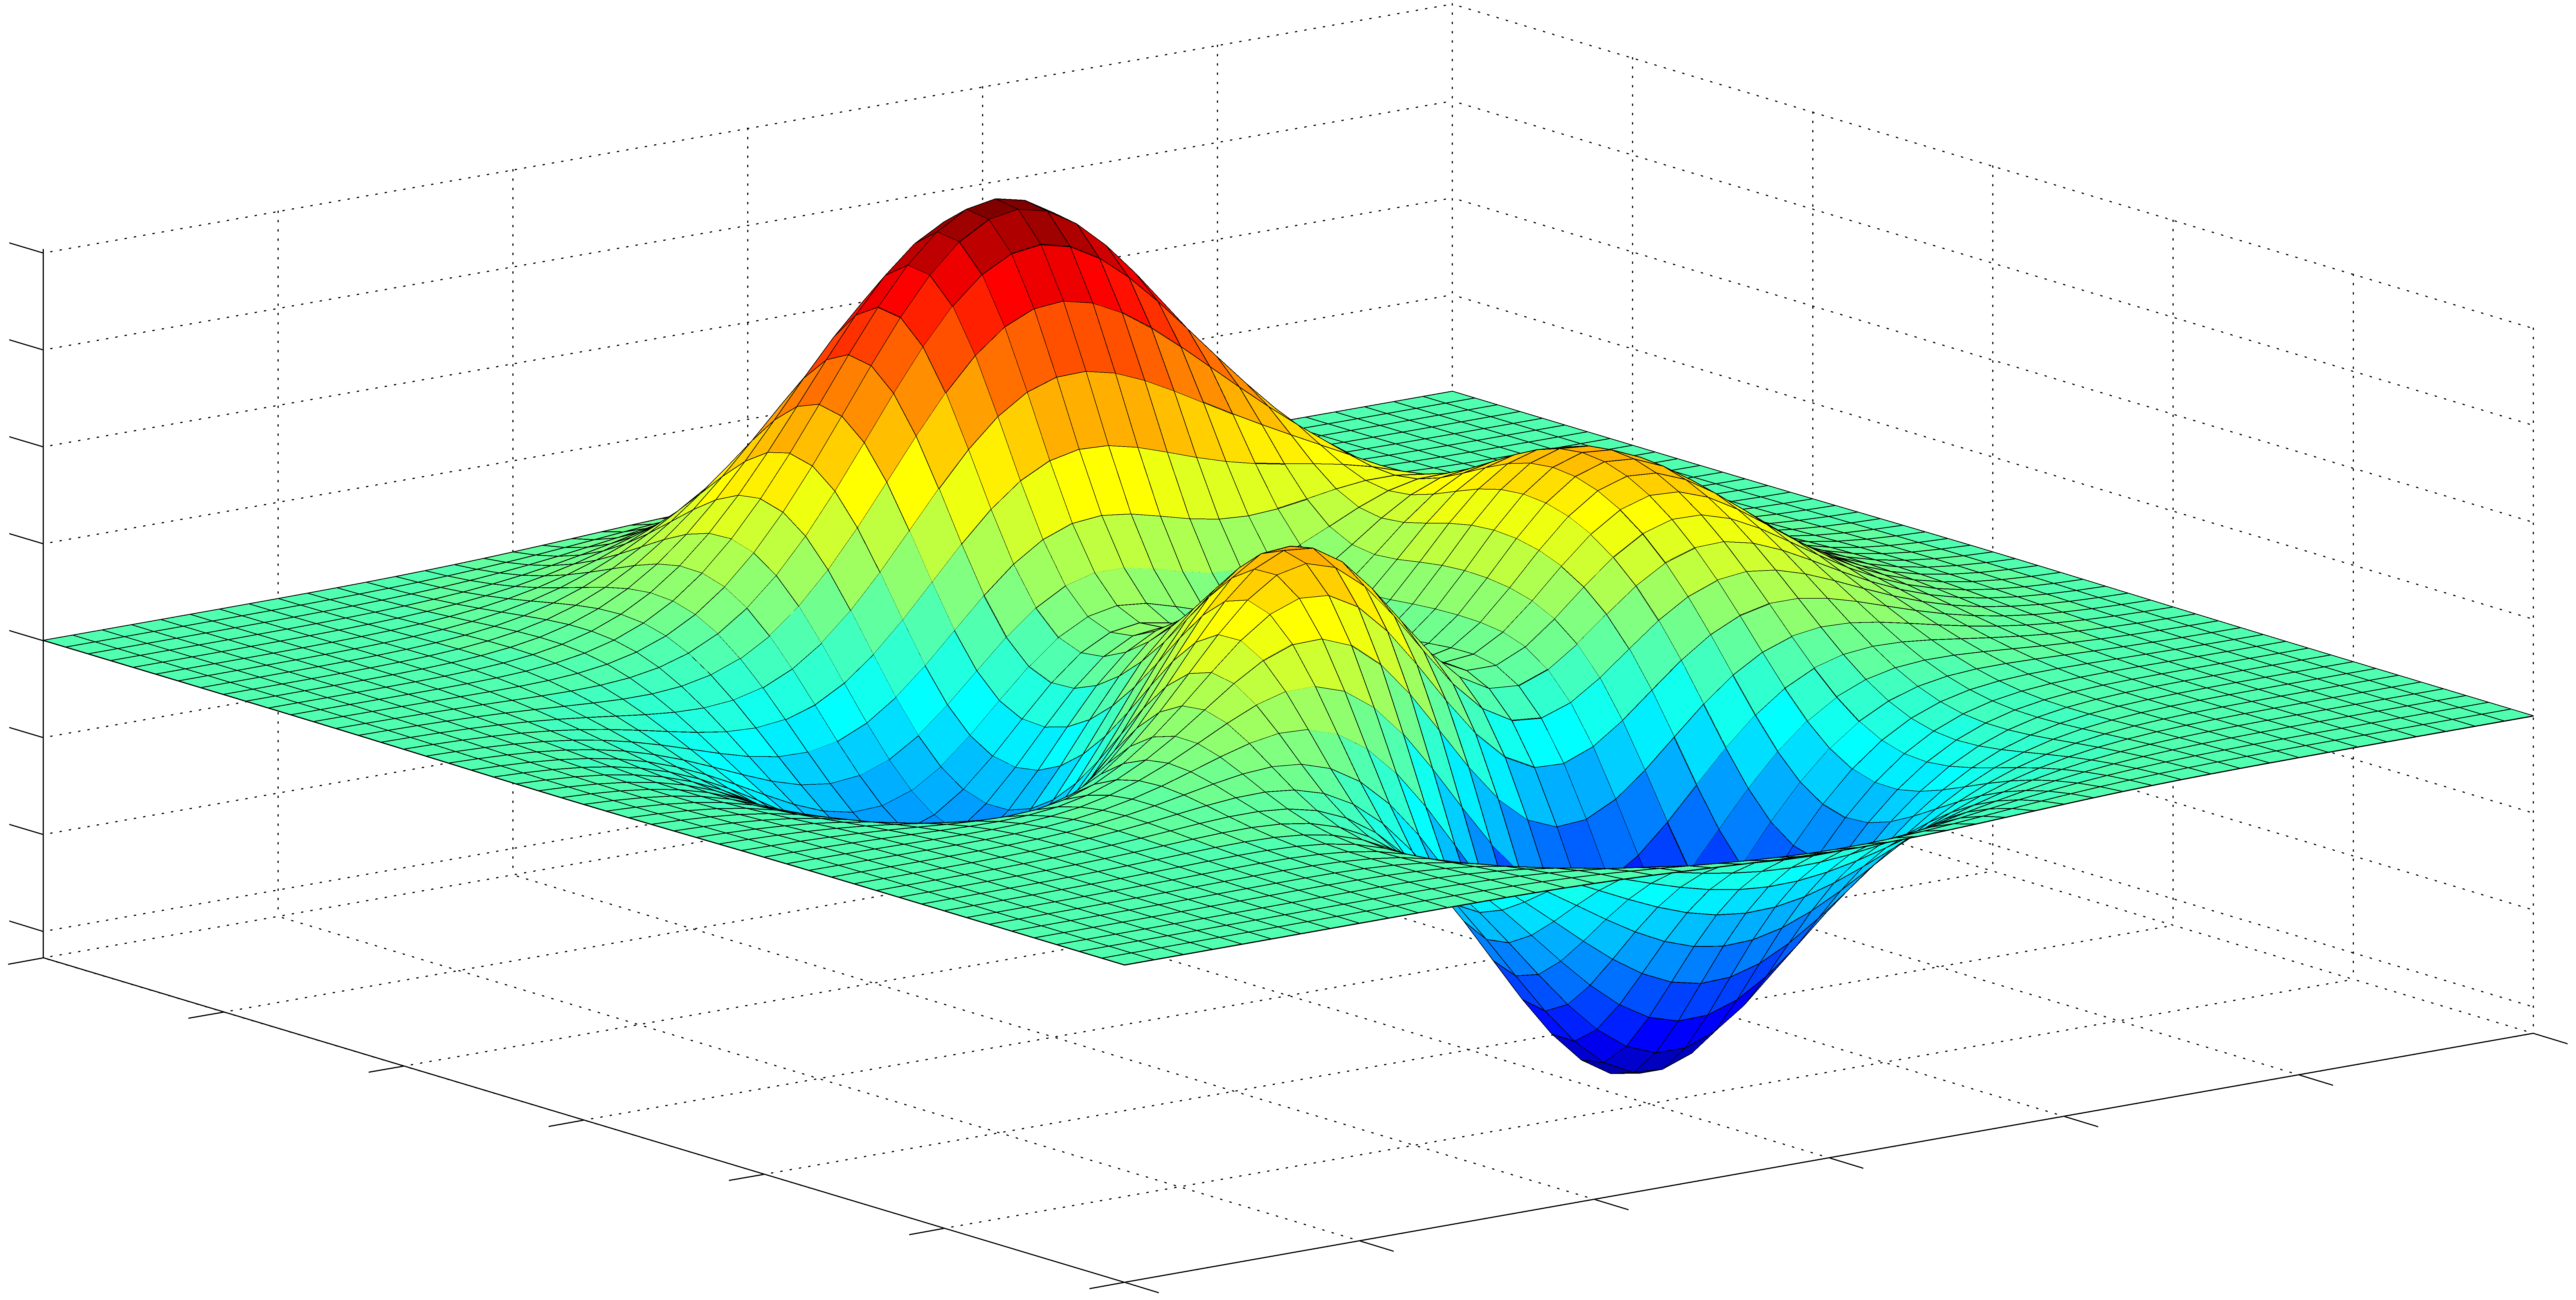
\includegraphics[width=18cm]{img/peaks.png}};
    \node at (2.4,-5.5) {\begin{minipage}{0.5\textwidth} \textbf{{\fontsize{50}{60}\selectfont MATLAB}}\\\fontsize{40}{50}\selectfont AVANÇADO\end{minipage}};
    \draw[rectangle, fill] (-3,-3) -- (10.75,-3) -- (10.75,-2.9) -- (-3,-2.9);
    \draw[rectangle, fill] (-3,-7.5) -- (10.75,-7.5) -- (10.75,-7.55) -- (-3,-7.55);
    \node at (2.55,-8.6) {\fontsize{25}{35}\selectfont Melissa Weber Mendonça};
    \draw[rectangle, fill] (-3,-9.5) -- (10.75,-9.5) -- (10.75,-9.55) -- (-3,-9.55);
    \draw[rectangle, fill] (-10.8,-25.5) -- (10.75,-25.5) -- (10.75,-27.55) -- (-10.8,-27.55);
    \node[color=white] at (-1.8,-26.6) {\fontsize{20}{30}\selectfont \textbf{UFSC}};
  \end{tikzpicture}
\end{center}

\clearpage

\restoregeometry
\pagestyle{plain} % No headers, just page numbers
\setcounter{page}{2}
\tableofcontents

\chapter{Estruturas de dados e MATLAB Básico}
%
\section{Revisão}
Vamos rever alguns conceitos básicos para a programação em MATLAB.

\begin{center}
  \begin{figure}[!ht]
  \begin{tikzpicture}
    \node[anchor=south west,inner sep=0] at (0,0) {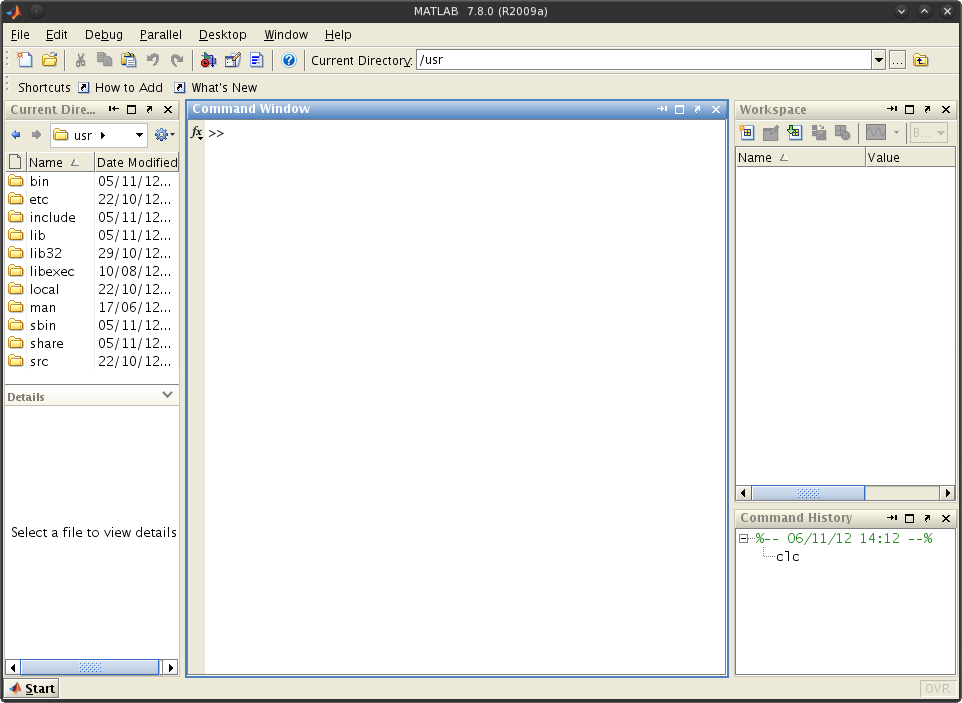
\includegraphics[width=0.6\textwidth]{img/matlab.png}};
    \node at (5,3) {Console};
    \node[text width=2cm] (ws) at (10.3,3.6) {Espaço de trabalho};
    \node (arq) at (-1,3) {Arquivos};
    \node (hist) at (10,1) {Histórico};
    \node (atual) at (6,7) {Diretório Atual};
    \draw[->, thick] (5.8,6.7) -- (5.4,6);
    \draw[->, thick] (arq) -- (-0.1,3.9);
    \draw[->, thick] (ws) -- (8.0,3.6);
    \draw[->, thick] (hist) -- (8,1);
  \end{tikzpicture}
  \caption{Janela de trabalho do MATLAB (varia de acordo com a versão instalada)}
  \end{figure}
\end{center}

\subsection{Console e scripts}
Para realizar tarefas simples no MATLAB, podemos usar diretamente o \emph{console}, digitando os comandos e obtendo as respostas. Se tivermos uma sequência de comandos a serem executados, podemos salvar estes comandos, em ordem, e um arquivo de extensão \code{.m} chamado \emph{script}. Em seguida, podemos digitar o nome deste arquivo no console, sem a extensão \code{.m}, tomando cuidado para que isso seja feito dentro do diretório em que o arquivo foi salvo. Assim, se temos um \emph{script} \code{arquivo.m} salvo no diretório atual, podemos executar os comandos contidos neste script digitando no console
\codigotikz{>> & arquivo}
e em seguida acionando a tecla \emph{Enter}.

\subsection{Atribuição}
Para determinarmos uma variável e atribuir um valor a ela no MATLAB, basta digitarmos 
\codigotikz{>> & variavel = valor}
(não é preciso declarar variáveis no MATLAB).

Assim, para criar diferentes tipos de variável, usamos os seguintes comandos:
\begin{itemize}
  \item Números (inteiros ou reais): 
    \codigotikz{>> & a = 1\\>> & b = 3.14}
  \item Vetores: as entradas devem estar separadas por vírgulas, espaços ou ponto-e-vírgula, dependendo da dimensão desejada para o vetor. Por exemplo, 
    \codigotikz{>> & v = [1,2,3]\\>> & v = [1 2 3]}
    definem um vetor com uma linha e três colunas; já 
    \codigotikz{>> & u = [1;2;3]}
    define um vetor com três linhas e uma coluna.
  \item Matrizes: para definir uma matriz, entre com as entradas por linhas, separando as linhas (que devem ter todas o mesmo número de colunas) por ponto-e-vírgula. Exemplo: 
    \codigotikz{>> & A = [1 2 3;4 5 6]}
  \item Texto: o valor de uma variável de texto deve ser sempre informado entre aspas.
    \codigotikz{>> & texto = 'Aqui vai meu texto.'}
\end{itemize}

Observe que para que o MATLAB execute o comando sem mostrar o resultado no console, basta acrescentarmos ponto-e-vírgula ao final da linha:
\codigotikz{>> & A = [1 2 3;4 5 6]\\
A = &\\
&1\; 2\; 3\\
&4\; 5\; 6\\
>> & A = [1 2 3;4 5 6];}

Além disso, para que o MATLAB exiba o valor de uma variável, basta digitarmos o nome da variável no console e em seguida pressionar \emph{Enter}:
\codigotikz{>> & A\\
A = &\\
& 1\; 2\; 3\\
& 4\; 5\; 6}

Já para mostrarmos mensagens de texto no MATLAB, usamos o comando \code{disp}:
\codigotikz{>> & disp('Olá!')}

Para entrarmos com comandos longos, separando-os em várias linhas, podemos usar \code{...}:
\codigotikz{>> & soma = 1+2+3+4+5 ...\\
& \qquad +6+7+8+9+10\\
ans =& \\
& 55}

\subsection{Matrizes}
	
No MATLAB, \emph{todas as variáveis são matrizes}. Isso significa que todas as variáveis podem ser acessadas através de índices de linha e coluna, informados nesta ordem, entre parênteses e separados por vírgula. É importante lembrar que no MATLAB todas as variáveis são indexadas a partir do índice \code{1}.

Para acessarmos os elementos de uma variável, usamos a sintaxe do seguinte exemplo:
\codigotikz{>> & v = [5;6;7]\\
  >> & v(1)\\
  ans = &\\
  & 5\\
  >> & v(2,1)\\
  ans = &\\
  & 6\\
  >> & A = [1 0 2;3 6 5;5 3 4]\\
  >> & A(1,2)\\
  ans = &\\
  & 0\\
  >> & numero = 2\\
  >> & numero(1)\\
  ans = & \\
  & 2\\
  >> & numero(1,1)\\
  ans = & \\
  & 2}	

\paragraph*{Observação.} O MATLAB permite que se acesse os elementos de uma matriz usando um índice único; nesse caso, os elementos são acessados da seguinte maneira:
\begin{equation*}
  A(i+m(j-1)) = A(i,j),
\end{equation*}
com $1\leq i \leq m$, $1\leq j\leq n$, $A\in {\mathbb{R}}^{m\times n}$.

\subsection{Comandos básicos}
Em seguida, listamos alguns comandos básicos do MATLAB.
\begin{itemize}
  \item \code{eye(n,n)} (ou \code{eye(n)}) cria uma matriz identidade de dimensão $n\times n$.
  \item \code{zeros(m,n)} cria uma matriz de zeros de dimensão $m\times n$.
  \item \code{ones(m,n)} cria uma matriz de números 1 de dimensão $m\times n$.
  \item \code{rand(m,n)} cria uma matriz de dimensão $m\times n$ com entradas aleatórias (com valor entre 0 e 1).
  \item \code{size(A)} retorna um vetor contendo as dimensões da variável $A$ (que pode ser um número, um vetor, uma matriz ou um texto).
  \item \code{length(A)} retorna o comprimento da maior dimensão da variável $A$ (se $A$ for uma matriz $m$ por $n$, com $m\geq n$, o resultado será $m$).
  \item \code{inv(A)} calcula a matriz inversa da matriz $A$.
  \item \code{k*a} calcula o produto de $k$ por cada elemento de $a$. Se $a$ for um vetor, ou uma matriz, o resultado é uma variável de mesma dimensão de $a$, com seus respectivos elementos multiplicados por $k$.
  \item \code{a*b} retorna o produto de dois escalares $a$ e $b$, ou multiplica duas matrizes (ou dois vetores), caso tenham dimensão compatível, usando a fórmula de produto de matrizes que já conhecemos.
  \item \code{a.*b} multiplica \emph{os elementos} de quaisquer duas variáveis de mesmo tamanho $a$ e $b$. Exemplo: 
    \codigotikz{>> & a = [1;2;3]\\
      >> & b = [4;5;6]\\ 
      >> & a.*b \\
      ans = &\\& $\begin{matrix} 4\\10\\18\end{matrix}$}
  \item \code{a/b} divide o número $a$ pelo número $b$ ($b\ne 0$). Se $a$ e $b$ forem matrizes de dimensão compatível, isso é o mesmo que calcular $a*inv(b)$.
  \item \code{a./b} divide \emph{os elementos} de quaisquer duas variáveis de mesmo tamanho $a$ e $b$. Exemplo: 
    \codigotikz{>> & a = [1;2;3]\\ >> & b = [4;5;6]\\ >> & a./b \\ans = &\\& $\begin{matrix} 1/4\\2/5\\3/6\end{matrix}$}
  \item \code{a\^{}k} calcula $a^k$, se $a$ for um número ou uma matriz.
  \item \code{a.\^{}k} eleva cada um dos elementos da variável $a$ (que pode ser de qualquer tipo) à $k$-ésima potência. Exemplo: 
    \codigotikz{>> & a = [1;2;3]\\>> & a.\^{}2 = [1;4;9]}
  \item \code{a'} (ou \code{transpose(A)}) calcula a transposta de $a$. Se $a$ for um número, isso é a mesma coisa que $a$; se $a$ for um vetor ou matriz, o resultado é o vetor transposto ou a matriz transposta.
  \item \code{reshape(A,m,n)} reorganiza os elementos da matriz em uma nova forma, com \code{m} linhas e \code{n} colunas.
\end{itemize}

\paragraph*{Observação} Um texto, no MATLAB, é tratado como uma matriz (ou um vetor). Pode-se calcular tamanho e acessar elementos por índices assim como fizemos com as matrizes numéricas. Exemplo:
\codigotikz{>> & texto = 'Palavra'\\
>> & texto(1)\\
ans = & \\
& 'P'\\
>> & size(texto)\\
ans = &\\
& 1 \qquad 7\\
>> & texto'\\
ans = &\\
& P\\
& a\\
& l\\
& a\\
& v\\
& r\\
& a}

\subsection{Acessando submatrizes: \emph{Slicing}}

O MATLAB oferece uma maneira fácil de se acessar subelementos de matrizes, chamada \emph{slicing}. Nesta operação, usamos a sintaxe
\begin{center}
  \code{A(linhainicial:linhafinal, colunainicial:colunafinal)}
\end{center}
para acessar a submatriz determinada entre as linhas \code{linhainicial} e \code{linhafinal}, e entre as colunas \code{colunainicial} e \code{colunafinal}. Aqui, é preciso tomar cuidado para que as dimensões da matriz resultante sejam consistentes.

Exemplo:
\codigotikz{>> & A = [1 2 3;4 5 6;7 8 9];\\
>> & A(2,:)\\
ans = &\\
& 4\; 5\; 6\\
>> & A(:,3)\\
ans = &\\
& 3\\
& 6\\
& 9\\
>> & A(1:2,3)\\
ans = &\\
& 3\\
& 6}

Note que \code{A(:,:)} retorna a matriz original, e que \code{A(:)} retorna a matriz em formato vetor:
\codigotikz{>> A(:)\\
ans = & \\
& 1\\
& 4\\
& 7\\
& 2\\
& 5\\
& 8\\
& 3\\
& 6\\
& 9}

Usando slicing, podemos facilmente apagar elementos de matrizes (ou linhas/colunas inteiras) usando a seguinte sintaxe:
   
\codigotikz{>> & A(i,:) = []\\
>> & A(:,j) = []}

Podemos também acrescentar elementos a qualquer momento:
      
\codigotikz{>> & lista = [1,3,4,5]\\
  >> & lista = [lista 2]\\
  >> & lista}

\paragraph*{Observação} Como a sintaxe acima também se aplica a texto, podemos concatenar textos facilmente e usar slicing:

\codigotikz{>> & frase = 'Oi, como vai?'\\
  >> & frase = [frase(1:length(frase)-1) ' você?']\\
  >> & frase(1:2)}

\subsection{Controle de fluxo}

Para repetirmos um bloco de código várias vezes, usamos a estrutura \code{for}:
\codigotikz{for & \emph{variável} = \emph{início}:\emph{fim}\\
& \emph{comando}\\
end&}
Se quisermos determinar um passo diferente de 1 entre os valores \emph{início} e \emph{fim}, usamos a sintaxe
\codigotikz{for & \emph{variável} = \emph{início}:\emph{passo}:\emph{fim}\\
& \emph{comando}\\
end&}

Observe que estruturas de controle de fluxo podem ser escritas diretamente no console do MATLAB. 

Exemplo:
\codigotikz{>> & for i = 1:3\\
& \quad i\\
& end\\
i =& \\
& 1\\
i = &\\
& 2\\
i = &\\
& 3\\
>> & for i = 3:-1:1\\
& \quad i \\
& end\\
i =& \\
& 3\\
i = &\\
& 2\\
i = &\\
& 1}

Quando é necessário repetir certo comando de código várias vezes \emph{até que} uma certa condição lógica seja satisfeita, usamos a estrutura \code{while}:
\codigotikz{
>> & i = 1;\\
>> & while i < 3\\
& \quad disp('Mais um.')\\
& \quad i = i + 1;\\
& end}

Para executarmos um bloco de comandos apenas se uma determinada condição lógica for satisfeita, usamos a estrutura \code{if}:
\codigotikz{
& if (sentença lógica)\\
& \quad faça (1)\\
& else\\
& \quad faça (2)\\
& end}

Em Matlab, uma sentença lógica pode ter dois valores: \code{0} (Falso) ou \code{1} (Verdadeiro).

\paragraph*{Observação} Para atribuir um valor a uma variável usamos o símbolo \code{=}; para compararmos se dois valores são iguais, usamos o símbolo \code{==}.

Exemplo:
\codigotikz{>> & i = 2;\\
>> & if i == 1\\
& \quad disp('Um.')\\
& else\\
& \quad disp('Não é um...')\\
& end\\
& Não é um...\\
>> & i = 1;\\
>> & if i == 1\\
& \quad disp('Um.')\\
& else\\
& \quad disp('Não é um...')\\
& end\\
& Um.}

\section{Estruturas de dados heterogêneas: Células}

Muitas vezes, gostaríamos de armazenar dados \emph{heterogêneos}; por exemplo, poderíamos desejar armazenar uma tabela do tipo
\begin{center}
   \begin{tabular}{l c c}
      Título & Núm. Páginas & Datas de Empréstimo e Devolução\\\toprule
      ``Álgebra Linear'' & 205 & 12/08, 15/08\\
      ``Cálculo'' & 346 & 10/09, 12/09\\
      ``Geometria'' & 123 & 04/08, 05/09\\
      ``Topologia'' & 253 & 01/08, 04/09
   \end{tabular}
\end{center}

Porém, esses dados são de naturezas diferentes: misturamos texto (\emph{string}), números e intervalos. Como armazenar isso em uma só tabela no MATLAB? 

A estrutura de dados que possibilita esse armazenamento é chamada \emph{célula} (\textbf{\texttt{cell}}), e pode ser utilizada da seguinte maneira:
\codigotikz{>> & tabela = \{ 'Algebra Linear', 205, [1208, 1508];\\
& \hskip2.35cm 'Calculo', 346, [1009, 1209];\\
& \hskip2.35cm 'Geometria', 123, [0408, 0509];\\
& \hskip2.35cm 'Topologia', 253, [0108, 0409] \}}
As células no MATLAB funcionam como matrizes, mas os índices são dados sempre entre chaves. A diferença entre células e matrizes é que em uma matriz, todas as entradas devem ter o mesmo tipo de dados; em uma célula, podemos misturar tipos diferentes de dados.

Como as células podem conter uma variedade de tipos de dados, nem sempre conseguimos acessar os valores diretamente pelo console. Por exemplo, 
\codigotikz{>> & tabela\\
tabela = & \\
& \begin{tabular} {l c c}
  'Algebra Linear' & [205] & [1x2 double]\\
  'Calculo' & [346] & [1x2 double]\\
  'Geometria' & [123] & [1x2 double]\\
  'Topologia' & [253] & [1x2 double]
\end{tabular}}

Assim, para vermos exatamente o que está armazenado na variável \code{tabela}, basta usarmos o comando
\codigotikz{>> & celldisp(tabela)}

Outros comandos válidos:
\begin{itemize}
   \item Para verificar o tamanho de uma célula, usamos o comando
   \codigotikz{>> & size(tabela)}
   \item Para criar uma célula vazia com $m$ por $n$ elementos, usamos o comando
   \codigotikz{>> & tabela = cell(m,n)}
   \item É possível transpor uma célula usando a mesma notação que usamos para matrizes:
     \codigotikz{>> & tabela'\\
       >> & transpose(tabela)}
%   \item Para apagar um elemento da célula, podemos usar a notação de matriz vazia:
%   \codigotikz{>> & tabela\{1,2\} = []}
%   \item É possível usar \emph{slicing} e transpor uma célula, como se fosse uma matriz.
%     \codigotikz{>> & tabela{1,:}}
\end{itemize}

\subsection{Acessando dados dentro de uma célula}

Existem duas maneiras de acessar elementos dentro de uma célula:
\begin{itemize}
\item Se usamos índices entre parênteses, estamos acessando um subconjunto da célula original.
\item Se usamos chaves (\code{\{\}}), estamos acessando os valores no interior de cada elemento da célula.
\end{itemize}

Exemplo:
\codigotikz{>> & sub = tabela(1:2,1:2)\\
sub = & \\
& \begin{tabular}{l c}
  'Algebra Linear' & [205]\\
  'Calculo' & [346]
  \end{tabular}\\
>> & tabela(2,:) = \{'MATLAB', 300, [1201, 1401]\};\\
>> & tabela\\
tabela = & \\
& \begin{tabular} {l c c}
  'Algebra Linear' & [205] & [1x2 double]\\
  'MATLAB' & [300] & [1x2 double]\\
  'Geometria' & [123] & [1x2 double]\\
  'Topologia' & [253] & [1x2 double]
\end{tabular}}

Note que mesmo as células que contêm valores numéricos não estão armazenadas como números. Repare nos colchetes:
\codigotikz{>> & vetor = tabela(:,2)\\
vetor = & \\
& \begin{tabular}{c}
  [205]\\ \relax
  [300]\\ \relax
  [123]\\ \relax
  [253]
\end{tabular}\\
>> & 3*vetor\\
& \emph{Undefined function 'mtimes' for input}\\
& \emph{ arguments of type 'cell'.}}

Podemos facilmente converter esses dados para uma variável numérica usando o comano \code{cell2mat}:
\codigotikz{>> & vetor = cell2mat(tabela(:,2))\\
vetor = & \\
& \begin{tabular}{c}
  205\\
  300\\
  123\\
  253
\end{tabular}\\
>> & 3*vetor\\
ans = & \\
& \begin{tabular}{c}
  615\\
  900\\
  369\\
  759
\end{tabular}}

Para acessarmos o conteúdo de uma célula individual, usamos as chaves. Por exemplo, na nossa tabela, 
\codigotikz{>> & tabela\{1,1\}}
é um texto com valor \code{'Algebra Linear'}, enquanto que 
\codigotikz{>> & tabela\{1,2\}}
é um número de valor $205$.

O resultado de um acesso simultâneo a várias células, por exemplo usando slicing, é uma \emph{lista} de valores:
\codigotikz{>> & tabela\{1:3,2\}\\
ans =& \\
& 205\\
ans = & \\
& 300\\
ans = & \\
& 123}
Note que se fizermos
\codigotikz{>> & teste = tabela\{1:3,2\}}
a variável \code{teste} conterá apenas o primeiro resultado da operação!

Para armazenarmos todo o resultado do acesso a estes valores da célula, podemos associar o resultado a uma lista com o mesmo número de elementos que o número de resultados do acesso:
\codigotikz{>> & [a,b,c] = tabela\{1:3,2\}\\
a = & \\
&    205\\
b =& \\
&    300\\
c =& \\
&    123}

Se todos os elementos selecionados da célula possuirem o mesmo tipo de dados, podemos atribuir esses elementos selecionados a uma só variável. Por exemplo, neste caso todos os dados selecionados são números, e assim:
\codigotikz{>> & numpaginas = [tabela\{1:3,2\}]\\
numpaginas = &\\
& 205 \; 346 \; 123}

No nosso exemplo, também temos variáveis de texto dentro da primeira coluna da célula. Podemos acessar um subconjunto do texto contido em uma das células associando os respectivos índices. Por exemplo:
\codigotikz{>> & tabela\{1,1\}(1:3)\\
ans = & \\
& 'Alg'}

Podemos construir estruturas de dados multidimensionais e heterogêneas, inclusive incluindo uma célula dentro de outra.

Exemplo:
\codigotikz{>> & v = \{ \{ 1, 'teste', [1;2] \};\\
  & \hskip1.3cm \{ [0,3], 12, 'nome', rand(4,4) \} \}}

Neste caso, os elementos devem ser referenciados da seguinte forma:
\codigotikz{>> & v\{2\}\{1\}}

Podemos, analogamente ao que fizemos com vetores, concatenar células:
\codigotikz{>> & C1 = \{'Joao', 16\};\\
  >> & C2 = \{'Maria', 18; 'Ricardo', 13\};\\
  >> & cola = \{C1 C2\}\\
  >> & uniao = [C1; C2]}

\section{Estruturas de dados heterogêneas: \emph{Structs}}

Outra maneira de armazenar dados heterogêneos é usar \emph{structs}: cada struct é composta de campos que podem conter quaisquer tipos de dados (assim como as células), e que são referenciados por \emph{nome}. Para criarmos uma struct chamada \code{dados} com o campo chamado \code{Nome}, podemos usar diretamente a sintaxe
\codigotikz{>> & dados.Nome = 'Melissa'\\
>> & dados.Sobrenome = 'Mendonça'}
ou
\codigotikz{>> & dados = struct('Nome', 'Melissa', ...\\
& \qquad 'Sobrenome', 'Mendonça')}
Nestes casos, a struct \code{dados} conterá um \emph{campo} chamado \code{Nome} e outro chamado \code{Sobrenome}; podemos armazenar em cada elemento da struct \code{dados} valores para estes campos; assim, isso significa que
\codigotikz{>> & dados(1).Nome}
retorna o valor \code{'Melissa'}.
Observe os exemplos:
\codigotikz{>> & dados = struct('Nome', 'Melissa', ...\\
 & \qquad 'Sobrenome', 'Mendonça')\\
>> & dados(1)\\
ans = &\\
& \begin{tabular}{r l}
  Nome: & 'Melissa'\\
  Sobrenome: & 'Mendonça'
\end{tabular}\\
>> & dados(1).Nome\\
ans = & \\
& Melissa\\
>> & dados(2) = struct('Nome', 'Fulano', ...\\
& \qquad 'Sobrenome', 'Beltrano')\\
dados = & \\
& 1x2 struct array with fields:\\
& \quad Nome\\
& \quad Sobrenome\\
>> & dados(1)\\
ans = & \\
& \begin{tabular}{r l}
  Nome: & 'Melissa'\\
  Sobrenome: & 'Mendonça'
\end{tabular}\\
>> & dados(2)\\
ans = & \\
& \begin{tabular}{r l}
  Nome: & 'Fulano'\\
  Sobrenome: & 'Beltrano'
\end{tabular}\\
>> & dados.Nome\\
ans = & \\
& Melissa\\
ans = & \\
& Fulano\\
>> & [nome1, nome2] = dados.Nome\\
nome1 = & \\
& Melissa\\
nome2 = & \\
& Fulano}

Para criarmos uma struct vazia, podemos usar o comando
\codigotikz{>> & vazia = struct([])}

\subsection{Como lidar com os nomes dos campos}

As structs possuem campos nomeados, o que pode tornar mais fácil acessar os dados armazenados nesse tipo de variável. Alguns comandos do MATLAB permitem fazer isso.

\begin{itemize}
\item O comando \code{fieldnames(s)} permite recuperar em uma célula a lista dos nomes dos campos da struct \code{s}.
\item O comando \code{s = orderfields(s1)} ordena os campos da struct \code{s1} de modo que a nova struct \code{s} tem os campos em ordem alfabética.
\item O comando \code{s = orderfields(s1, s2)} ordena os campos da struct \code{s1} de forma que a nova struct \code{s} tenha os nomes dos campos na mesma ordem em que aparecem na struct \code{s2} (as structs \code{s1} e \code{s2} devem ter os mesmos campos).
\item O comando \code{s = orderfields(s1, c)} ordena os campos em \code{s1} de forma que a nova struct \code{s} tenha campos na mesma ordem em que aparecem na célula \code{c} (a célula \code{c} deve conter apenas os nomes dos campos de \code{s1}, em qualquer ordem).
\end{itemize}

\subsection{Structs e células}

Podemos preencher uma struct usando um comando só, determinando os valores possíveis para cada campo através de células. Por exemplo, no caso anterior, poderíamos ter entrado o comando
\codigotikz{>> & dados = struct('Nome', \{'Melissa', 'Fulano'\}, ...\\
& \qquad 'Sobrenome', \{'Mendonça', 'Beltrano'\})}
para criar a mesma struct.

Se quisermos preencher vários campos com o mesmo valor, não precisamos nos repetir. Por exemplo, 
\codigotikz{>> & dados = struct('Nome', \{'Melissa', 'Fulano'\}, ...\\
& \qquad 'Sobrenome', \{'Mendonça', 'Beltrano'\}, ...\\
& \qquad 'Presentes', \{'sim'\})}
gera uma struct com os dados
\codigotikz{&dados(1) = \\
& \begin{tabular}{r l}
  Nome: & 'Melissa'\\
  Sobrenome: & 'Mendonça'\\
  Presentes: & 'sim'
\end{tabular}\\
& dados(2) = \\
& \begin{tabular}{r l}
  Nome: & 'Fulano'\\
  Sobrenome: & 'Beltrano'\\
  Presentes: & 'sim'
\end{tabular}}

\subsection{Convertendo dados}

Existem duas funções do MATLAB que nos permitem converter dados de células para structs ou de structs para células.

O comando
\codigotikz{>> & s = cell2struct(\rm\emph{célula}, \rm\emph{campos}, \rm\emph{dimensão)}}
cria uma struct \code{s} a partir de uma célula \code{c}, de forma que os dados dispostos ao variarmos a dimensão escolhida possam ser distribuídos nos campos correspondentes informados no comando.

Exemplo:
\codigotikz{>> & tabela = \{'Melissa', 'Mendonça', 'sim';\\
& \qquad 'Fulano', 'Beltrano', 'sim'\}\\
tabela = & \\
& \begin{tabular}{l l l}
  'Melissa' & 'Mendonca' & 'sim'\\
  'Fulano' & 'Beltrano' & 'sim'
\end{tabular}\\
>> & campos = \{'Nome', 'Sobrenome', 'Presente'\};\\
>> & s = cell2struct(tabela, campos, 2);\\
s = & \\ 
& 2x1 struct array with fields:\\
& \quad Nome\\
& \quad Sobrenome\\
& \quad Presente\\
>> & s(1)\\
ans = & \\
& \begin{tabular}{r l}
         Nome: &'Melissa'\\
    Sobrenome: &'Mendonça'\\
     Presente: &'sim'
\end{tabular}\\
>> & s(2)\\
ans = & \\
& \begin{tabular}{r l}
         Nome: &'Fulano'\\
    Sobrenome: &'Beltrano'\\
     Presente: &'sim'
\end{tabular}}

Por outro lado, o comando
\codigotikz{>> & célula = struct2cell(\rm\emph{struct})}
cria uma célula a partir da estrutura \emph{struct}.

Exemplo:
\codigotikz{>> & celula = struct2cell(s)\\
celula = & \\
& \begin{tabular}{l l}
    'Melissa'  &    'Fulano'  \\
    'Mendonça' &   'Beltrano'\\
    'sim'      &    'sim'
\end{tabular}}

%%%%%%%%%%%%%%%%%%%%%%%%%%%%%%%%%%%%%
%%%%%%%%%%%%%%%%%%%%%%%%%%%%%%%%%%%%%
%GALLERY
%%%%%%%%%%%%%%%%%%%%%%%%%%%%%%%%%%%%%
%%%%%%%%%%%%%%%%%%%%%%%%%%%%%%%%%%%%%
\section{Funções}

No MATLAB, uma função é um arquivo \code{minhafuncao.m} com a sintaxe

\file{0.5\textwidth}{minhafuncao.m}{\begin{tabular}{l l} function & [y] = minhafuncao(x)\\
        & \% Descricao da funcao\\
        & comandos;\end{tabular}} 

Uma vez construida a função, podemos chamá-la no console, usando
\codigotikz{>> & y = minhafuncao(x)}

\paragraph*{Observação.} Uma função deve sempre ter o mesmo nome que o arquivo no qual ela está salva.

Exemplo: Construir uma função que calcule o módulo de um número real $x$.

\file{0.5\textwidth}{modulo.m}{\begin{tabular}{ll}function & [y] = modulo(x)\\
    & if x < 0\\
    & \quad y = -x;\\
    & else\\
    & \quad y = x;\\
    & end\end{tabular}}

Para retornar mais de um argumento, ou para que a função tenha mais de um argumento de entrada, basta separar os valores por vírgulas.

Exemplo: O comando \code{size} é uma função que recebe como argumento de entrada uma variável e retorna um vetor com as dimensões desta variável:
   \codigotikz{>>& [m,n] = size(A)}

Se quisermos aplicar a mesma função a um conjunto de valores, basta colocarmos os valores em um vetor:

\codigotikz{>> & m = f([-2 1 3])}

Por fim, se uma função está definida com vários argumentos de saída mas não precisamos de todos estes argumentos, podemos usar o símbolo \textasciitilde. 

Exemplo:
\codigotikz{>> & [\textasciitilde,n] = size(rand(10,5));}

\subsection{Funções com número variável de argumentos}

O MATLAB possui alguns comandos que permitem verificarmos a quantidade de argumentos de entrada e de saída de uma função:
\begin{itemize}
  \item O comando \code{nargin}, executado dentro do corpo de uma função, retorna o número de argumentos de entrada para o qual a função está definida.
  \item O comando \code{nargin(f)}, em que \code{f} é uma função, retorna o número de argumentos de entrada da função \code{f}, e pode ser executado fora da função (inclusive no console).
  \item O comando \code{nargout}, executado dentro do corpo de uma função, retorna o número de argumentos de saída para o qual a função está definida.
  \item O comando \code{nargin(f)}, em que \code{f} é uma função, retorna o número de argumentos de saída da função \code{f}, e pode ser executado fora da função (inclusive no console).
\end{itemize}
Além disso, podemos definir funções com número variável de argumentos de entrada ou de saída, usando respectivamente os comandos \code{varargin} e \code{varargout}.

O comando \code{varargin} é uma variável de entrada utilizada na definição de uma função que permite que a função receba qualquer número de argumentos de entrada. Quando a função for executada, \code{varargin} (que deve ser o último argumento de entrada) será uma célula de tamanho 1 por $n$, onde $n$ é o número de argumentos de entrada que a função recebeu além daqueles explicitamente declarados na função.

Exemplo:
\file{0.7\textwidth}{somas.m}{\begin{tabular}{ll}function & [y] = somas(x,varargin)\\
    & if nargin == 1\\
    & \quad disp('Nada a calcular.')\\
    & elseif nargin == 2\\
    & \quad y = x + varargin\{1\};\\
    & elseif nargin == 3\\
    & \quad y = x + varargin\{1\} + varargin\{2\};\\
    & else\\
    & \quad disp('Argumentos demais!')\\
    & end\end{tabular}}

O comando \code{varargout} é uma variável de saída utilizada na definição de uma função que permite que a função devolva qualquer número de argumentos de saída. Analogamente ao comando \code{varargin}, o comando \code{varargout} deve aparecer como o último argumento de saída na declaração da função, e é uma célula de tamanho 1 por $n$, em que $n$ é o número de argumentos de saída requisitados na execução da função além daqueles explicitamente declarados na função.

Exemplo:
\file{0.8\textwidth}{valores.m}{\begin{tabular}{l} function [f,varargout] = valores(x)\\
    \qquad f = x\^{}2;\\
    \qquad  if nargout == 2\\
    \qquad  \quad varargout\{1\} = 2*x;\\
    \qquad elseif nargout == 3\\
    \qquad \quad varargout\{1\} = 2*x;\\
    \qquad \quad varargout\{2\} = 2;\\
    \qquad elseif nargout > 3\\
    \qquad \quad disp(['Esta funcao calcula apenas f, derivada ' ...\\
    \qquad \qquad \qquad \qquad 'de f e segunda derivada de f.'])\\
    \qquad end\end{tabular}}

\subsection{Funções anônimas}

Suponha que queremos declarar uma função no console, sem ter que guardá-la em um arquivo. Por exemplo, queremos avaliar a função $f(x) = \sin{x}$ em alguns pontos. Para isto, podemos usar o conceito de \emph{função anônima}. 

Para definirmos uma \emph{função anônima}, usamos a seguinte sintaxe:
\codigotikz{>> & f = @(x) sin(x)}
e, em seguida, podemos avaliar a função, usando o comando
\codigotikz{>> & x = pi;\\
  >> & f(pi)}

Esta definição é bastante útil quando queremos passar uma função como argumento para outra função: por exemplo, para calcularmos o valor mínimo de uma função avaliada em 3 pontos distintos, podemos definir a função como uma função anônima, e em seguida passar o seu \emph{handle} como argumento para a função que calcula o mínimo entre os valores:

\codigotikz{>> & f = @(x) x-1;\\
   >> & min(f([-2 1 0]))}

Se quisermos criar uma função anônima com mais de uma variável, usamos 

\codigotikz{>> & f = @(x,y,z,t) x+y+z+t}

Para retornarmos mais de um valor de uma função anônima, usamos o comando \emph{deal}:

\codigotikz{>> & f = @(t,u,v) deal(t+u+v,t-u+2*v)\\
>> & [a,b] = f(1,2,3)}

% str2func
% func2str

\chapter{Gráficos em 2D e 3D}

\section{Gráficos em 2D}

Cada ponto no gráfico é dado por uma coordenada $(x,y)$, onde $x$ é um número real e $y$ é um número real associado a $x$ (como $y = f(x)$). Mas, não podemos representar a reta real (\emph{contínua}) no MATLAB. Por isso, precisamos definir um \emph{vetor} de pontos em um determinado intervalo (em $\mathbb{R}$ ou ${\mathbb{R}}^2$):
\begin{equation*}
   x = (x_1, x_2, \ldots, x_n)
\end{equation*}
e calcular o valor de $f$ apenas nestes pontos; o MATLAB ligará os pontos para desenhar o gráfico.

\subsection{Comando \code{plot}}

Para fazer gráficos simples em 2D (no plano), inicialmente precisamos definir o intervalo a ser utilizado para desenhar o gráfico. Para isso, precisamos de 3 argumentos:
\codigotikz{ >> & x = a:delta:b}
Aqui, \code{a} é a extremidade esquerda do intervalo; \code{b} é a extremidade direita do intervalo; e \code{delta} é o espaçamento desejado entre cada subintervalo, e determina assim o número total de pontos neste intervalo. O resultado, \code{x}, é um \emph{vetor} de pontos (que pode ser um vetor linha ou um vetor coluna).

\paragraph*{Observação} Analogamente, podemos usar o comando \code{linspace} para termos controle direto sobre o número de pontos desejados no intervalo:
\codigotikz{>> & y = linspace(a,b,n)}
gera um vetor de pontos $y$ com extremidade esquerda \code{a}, extremidade direita \code{b} e \code{n} pontos no total.
 
Em seguida, chamamos o comando 
\codigotikz{>> & plot(x,y)} 
onde \code{x} é o vetor de pontos no intervalo desejado, e \code{y} é um vetor dos valores da função a ser desenhada nos pontos do intervalo.

Exemplo:
  Para fazermos o gráfico da função $f(x) = x^2$ no intervalo $[-4,4]$, usamos os seguintes comandos:
  \codigotikz{
    >> & x = -4:0.5:4\\
    >> & y = x.\^{}2\\
    >> & plot(x,y)
  }	
  Desta forma, 
  $$x = (-4, -3.5,-3,-2.5,-2,-1.5,-1,-0.5,0,0.5,1,1.5,2,2.5,3,3.5,4)$$
  $$y = (16, 12.25,9,6.25,4,2.25,1,0.25,0,0.25,1,2.25,4,6.25,9,12.25,16)$$

\paragraph*{Algumas opções do comando {\code{plot}}}
Outras opções, como espessura da linha ou cor do desenho, podem ser especificadas no comando plot. 

Exemplo: 
  \codigotikz{>> & plot(x,y,'r*')\\
    >> & plot(x,y,'m\^{}')}

A lista de opções pra o comando \code{plot} pode ser obtida no MATLAB ao digitarmos \code{help plot}. Um resumo se encontra na Tabelas \ref{tab:cores} e \ref{tab:linhas}.
\begin{center}
  \begin{table}[h!]
    \begin{center}
      \begin{tabular}{l l}
        \toprule
        Símbolos & Cores\\\midrule
        \code{'k'} & Preto \\          
        \code{'r'} & Vermelho\\        
        \code{'g'} & Verde\\        
        \code{'b'} & Azul\\
        \code{'m'} & Rosa\\
        \code{'c'} & Azul claro\\
        \code{'y'} & Amarelo\\
        \code{'w'} & Branco\\\bottomrule
      \end{tabular}
    \end{center}
    \label{tab:cores}
    \caption{Cores.}
  \end{table}
\end{center}
\begin{center}
  \begin{table}[h!]
    \begin{center}
      \begin{tabular}{l l}
        \toprule
        Símbolo & Estilo de linha\\\midrule
        \code{'-'} & Linha contínua\\
        \code{'--'} & Linha tracejada\\
        \code{':'} & Pontilhado\\
        \code{'-.'} & Traço e ponto\\
        \code{'.'} & Pontos\\
        \code{'+'} & Cruzes\\
        \code{'*'} & Asteriscos\\
        \code{'o'} & Círculos\\
        \code{'x'} & X\\
        \code{'\^{}'} & Triângulos\\
        \code{'v'} & Triângulos\\
        \code{'>'} & Triângulos\\
        \code{'<'} & Triângulos\\
        \code{'s'} & Quadrados\\
        \code{'d'} & Losangos\\
        \code{'p'} & Pentágonos\\
        \code{'h'} & Hexágonos\\
        \bottomrule
      \end{tabular}
      \label{tab:linhas}
      \caption{Estilos de linha.}
    \end{center}
  \end{table}
\end{center}

\paragraph*{Observação} Note que se usarmos o comando \code{plot} sem especificar o estilo de linha, ou se usarmos o estilo padrão (\code{'-'}), o resultado será uma curva, enquanto que se utilizarmos as outras opções, teremos um desenho do conjunto dos pontos $x$ e $y$ desejados. Assim, podemos desenhar também conjuntos discretos sem maiores complicações.

Para modificar a espessura da linha, usamos a propriedade \code{'Linewidth'}:
\codigotikz{>> & plot(x,y,'Linewidth',2)}

Para mais opções e propriedades dos gráficos, consulte o \emph{help} do MATLAB.

\paragraph*{Observação} Todos os comandos modificadores do gráfico que veremos adiante devem ser executados \emph{após} a criação do gráfico. Portanto, o primeiro passo para se fazer uma figura é sempre criar o gráfico básico (eixo), para depois acrescentar títulos, descrições, etc.

\paragraph*{Observação} Para fecharmos a janela de gráficos atual, usamos o comando \code{close}.

\subsubsection{Vários gráficos no mesmo eixo}
Para fazer mais de um gráfico no mesmo eixo, usamos os comandos \code{hold}. A utilização básica é a seguinte:
\codigotikz{>> & plot(x,y)\\
  >> & \bf{hold on}\\
  >> & plot(x,z)\\
  >> & \bf{hold off}
}
O comando \code{hold on} sinaliza ao MATLAB que ainda vamos fazer mais gráficos no mesmo eixo, enquanto que o comando \code{hold off} desliga essa opção. Portanto, qualquer gráfico feito após o comando \code{hold off} vai apagar o gráfico atual e substitui-lo em um novo eixo.

Exemplo:
  Representar graficamente o sistema linear abaixo:
  \begin{equation*}
    \left\{ 
      \begin{array}{l}
        x_1 + x_2 = 8\\
        4x_1 + 2x_2 = 26 
      \end{array} 
    \right. \Leftrightarrow \left\{ 
      \begin{array}{l} 
        x_2=8 - x_1\\
        x_2=13 - 2x_1
      \end{array} 
    \right.\Leftrightarrow 
    \begin{pmatrix}
      x_1\\x_2
    \end{pmatrix} = 
    \begin{pmatrix}
      5\\3
    \end{pmatrix}
  \end{equation*}
  \codigotikz{
    >> & x1 = 0:0.1:10\\
    >> & plot(x1,8-x1)\\
    >> & hold on\\
    >> & plot(x1,13-2*x1)\\
    >> & hold off
  }

\subsubsection{Título: \code{title}}
Para incluirmos um título em um gráfico produzido no MATLAB, basta usarmos o comando \code{title} \emph{após} a criação do gráfico:
\codigotikz{>> & title('y=f(x)')}

Exemplo:
  \codigotikz{>> & x = -pi:0.1:pi\\
    >> & plot(x,sin(x),'r')\\
    >> & title('Gráfico da função y=sin(x)')}

\subsubsection{Legendas nos eixos: \code{label}}
Para incluirmos legendas nos eixos do gráfico, usamos os comandos \code{xlabel} e \code{ylabel} para os eixos horizontal e vertical, respectivamente. Assim como o comando \code{title}, estes comandos também devem ser utilizados \emph{após} a criação do gráfico.

Exemplo:
  \codigotikz{>> & t = 0:0.1:10\\
    >> & p = exp(t)\\
    >> & plot(t,p)\\
    >> & title('Gráfico da pressão em função do tempo.')\\
    >> & xlabel('tempo')\\
    >> & ylabel('pressão')}

\subsubsection{Legendas dos gráficos: \code{legend}}
Para incluirmos nos gráficos legendas sobre cada linha que está sendo desenhada, usamos o comando \code{legend}, da seguinte forma:
\codigotikz{>> & x = -pi:0.1:pi\\
  >> & plot(x,sin(x))\\
  >> & title('Gráfico 1')\\
  >> & legend('y=sin(x)')}
Se temos mais de um gráfico no mesmo eixo, usamos o comando \code{legend} com os textos desejados nas legendas, \emph{na ordem em que os gráficos foram desenhados}:
\codigotikz{>> & legend('legenda 1','legenda 2','legenda 3')}

Exemplo:
  \codigotikz{>> & x = -2*pi:0.1:2*pi;\\
    >> & plot(x,sin(x))\\
    >> & hold on\\
    >> & plot(x,cos(x),'r')\\
    >> & legend('y=sin(x)','y=cos(x)')\\
    >> & title('Funções seno e cosseno.')}

\subsubsection{Eixos coordenados: \code{axis}}
Às vezes, precisamos fixar ou modificar os eixos coordenados nos quais fazemos os gráficos. Para isso, podemos usar o comando \code{axis} de várias formas.
\begin{itemize}
  \item \code{axis}: cria um ``eixo coordenado'' padrão.
  \item \code{axis([x0 x1 y0 y1])}: modifica os eixos coordenados da figura atual de maneira que o eixo horizontal começa em $x0$ e termina em $x1$, e o eixo vertical começa em $y0$ e termina em $y1$.
  \item \code{axis auto}: deixa o MATLAB tentar encontrar um eixo coordenado ideal para a imagem desenhada.
  \item \code{axis equal}: toma eixos coordenados na mesma escala.
  \item \code{axis tight}: toma eixos coordenados ``justos'' aos dados.
  \item \code{axis off}: não mostrar o eixo coordenado (\code{axis on} reverte esta ação)
\end{itemize}

\subsubsection{Malha: \code{grid}}
Podemos mostrar uma malha no nosso gráfico usando o comando \code{grid on}. Para revertermos este comando, basta usar \code{grid off}. Além disso, podemos também escolher uma malha mais refinada usando \code{grid minor}.

Exemplo:
  \codigotikz{>> & t = 0:pi/20:2*pi\\
    >> & plot(sin(t),2*cos(t))\\
    >> & grid on\\
    >> & grid minor}

\subsection{Retas e segmentos: \code{line}}

Para desenharmos retas e segmentos de reta no MATLAB, podemos fazer o gráfico da reta usando sua equação na forma $y=ax+b$, no comando \code{plot}, ou podemos usar o comando \code{line}. Este comando toma como entrada as coordenadas dos pontos $p=(x0,y0)$ e $q=(x1,y1)$ que desejamos ligar pelo segmento de reta a ser desenhado:
\codigotikz{>> & line([x0 x1],[y0 y1])}

Exemplo:
  Para desenharmos o segmento que vai do ponto $p=(1,2)$ até o ponto $q = (3,4)$, usamos o comando
  \codigotikz{>> & line([1 3],[2 4])}

Se nos argumentos tivermos mais de dois pontos, o MATLAB gerará um conjunto de segmentos (ou um polígono) ligando os pontos em ordem.

Exemplo:
  Para desenharmos um triângulo ligando os pontos $(0,0)$, $(1,0)$ e $(0,1)$ no MATLAB, usamos o seguinte comando:
  \codigotikz{>> & line([0 1 0 0],[0 0 1 0])\\
    >> & axis([-1 2 -1 2])}
  (acrescentamos o comando \code{axis} no exemplo acima para podermos visualizar corretamente o triângulo.)

\subsection{Regiões preenchidas: \code{fill}}
   
Para desenharmos regiões preenchidas no MATLAB, usamos o comando \code{fill(X,Y,C)}, onde \code{X} e \code{Y} são um conjunto de coordenadas para os pontos $p1 = (X1,Y1)$, $p2 = (X2,Y2)$, etc e \code{C} é a cor desejada para o preenchimento (mesmas cores usadas no comando \code{plot}).

Exemplo:
  \codigotikz{>> & X = [0 1 0 0]\\
    >> & Y = [0 0 1 0]\\
    >> & fill(X,Y,'m')}

\subsection{Subgráficos: \code{subplot}}

Se quisermos fazer vários gráficos na mesma janela, podemos usar o comando \code{subplot}, da seguinte forma:
\codigo{>> & subplot(m,n,i), plot(x,y)}
desenha o gráfico determinado pelas coordenadas \code{x} e \code{y} na posição $i$ de uma matriz de gráficos com $m$ linhas e $n$ colunas. O índice dos gráficos é determinado da seguinte maneira: se temos, por exemplo, $8$ gráficos organizados em uma matriz com 2 linhas e 4 colunas, os gráficos serão desenhados na ordem abaixo:
\begin{equation*}
  \begin{array}{c c c c}
    1 & 2 & 3 & 4\\
    5 & 6 & 7 & 8
  \end{array}
\end{equation*}

Exemplo:
  Fazer em uma mesma janela os gráficos das funções seno, cosseno, tangente e cotangente entre $-2\pi$ e $2\pi$.
  \codigotikz{>> & x = -2*pi:0.01:2*pi;\\
    >> & subplot(2,2,1), plot(x,sin(x),'r')\\
    >> & subplot(2,2,2), plot(x,cos(x),'c')\\
    >> & subplot(2,2,3), plot(x,tan(x),'g')\\
    >> & subplot(2,2,4), plot(x,cot(x))}

\subsection{Curvas no espaço: \code{plot3}}
   
Se quisermos desenhar um conjunto de pontos ou uma curva parametrizada no espaço, podemos usar o comando \code{plot3}. O comando
\codigotikz{>> & plot3(X,Y,Z)}
desenha a curva determinada pelos pontos $(X,Y,Z)$ no espaço.

Exemplo:
  \codigotikz{>> & t = 0:pi/50:10*pi;\\
    >> & plot3(sin(t),cos(t),t)\\
    >> & xlabel('sin(t)')\\
    >> & ylabel('cos(t)')\\
    >> & zlabel('t')\\
    >> & axis square}

Também podemos usar a função plot3 para observar a distribuição de pontos no espaço.

Exemplo:
  \codigotikz{>> & x = rand(100,1);\\
    >> & y = rand(100,1);\\
    >> & z = rand(100,1);\\
    >> & plot3(x,y,z)}

\section{Gráficos em 3D}

O procedimento de criação de gráficos em 3D no MATLAB é bastante parecido com o procedimento para a criação de gráficos no plano. A maior diferença é a geração dos intervalos de pontos a serem desenhados e a variedade de tipos de gráfico que podemos fazer.

Neste caso, queremos o gráfico de uma função de duas variáveis, ou seja, uma superfície dada por
\begin{equation*}
   z = f(x,y)
\end{equation*}
%
\subsection{Criador de malha: \code{meshgrid}}

Aqui, ao invés de criarmos um intervalo de pontos onde o gráfico será desenhado, precisamos de uma \emph{malha}, ou seja, da intersecção de dois intervalos, um definido no eixo $x$ e outro definido no eixo $y$, para desenharmos uma função $z = f(x,y)$. Para isto, usamos a função \code{meshgrid}.
   
\codigotikz{>> & [X,Y] = meshgrid(x,y)}

cria matrizes \code{X} e \code{Y} prontas para serem usadas pelos comandos de criação de gráficos em 3D. 

As matrizes resultantes da função \code{meshgrid} são construidas da seguinte maneira. Se $x$ tem $n$ elementos e $y$ tem $m$ elementos, as matrizes \code{X} e \code{Y} tem ordem $m\times n$, e contém os elementos dos vetores \code{x} e \code{y} repetidos. Assim, se \code{x = [x1,x2,x3]} e \code{y = [y1,y2,y3,y4]}, então
\begin{equation*}
  X = \begin{pmatrix}
    x1 & x2 & x3\\
    x1 & x2 & x3\\
    x1 & x2 & x3\\
    x1 & x2 & x3
  \end{pmatrix}
\end{equation*}
e
\begin{equation*}
  Y = \begin{pmatrix}
    y1 & y1 & y1\\
    y2 & y2 & y2\\
    y3 & y3 & y3\\
    y4 & y4 & y4
  \end{pmatrix}
\end{equation*}
Desta forma, o MATLAB lê os dados das duas matrizes em pares, resultando em um conjunto de pontos da forma
\begin{equation*}
  \begin{pmatrix}
    (x1,y1) & (x2,y1) & (x3,y1)\\
    (x1,y2) & (x2,y2) & (x3,y2)\\
    (x1,y3) & (x2,y3) & (x3,y3)\\
    (x1,y4) & (x2,y4) & (x3,y4)
  \end{pmatrix}
\end{equation*}
e assim calcula todas as combinações dos pontos da malha.

Se queremos usar uma malha igualmente espaçada e definida no mesmo intervalo nos eixos $x$ e $y$, podemos usar o comando \code{meshgrid} com somente um argumento de entrada:

\codigotikz{>> & x = -1:0.1:1\\
  >> & [X,Y] = meshgrid(x)}

cria uma malha em $[-1,1]\times [-1,1]$ com espaçamento de $0.1$ unidades entre os pontos.
% 
\subsection{Superfícies}

Nesta seção, vamos ver os comandos que nos permitem desenhar superfícies no MATLAB. 

\subsubsection{Superfícies sólidas: \code{surf}}

Para desenharmos uma superfície dada por 
\begin{equation*}
   z = f(x,y)
\end{equation*}
com $(x,y) \in \Omega$, onde $\Omega$ é uma região do plano definida por $[x_0,y_0]\times [x_1,y_1]$, usamos o comando \code{surf(X,Y,Z)}.

\codigotikz{>> & x = x0:deltax:x1;\\
  >> & y = y0:deltay:y1;\\
  >> & [X,Y] = meshgrid(x,y);\\
  >> & Z = f(X,Y)\\
  >> & surf(X,Y,Z)}

Exemplo:
  \codigotikz{>> & x = -1:0.1:1;\\
    >> & [X,Y] = meshgrid(x);\\
    >> & Z = X.\^{}2+Y.\^{}2\\
    >> & surf(X,Y,Z)}

Exemplo:
  \codigotikz{>> & x = -3:0.1:3;\\
    >> & [x,y] = meshgrid(x);\\
    >> & f = @(x,y) x.\^{}2+3*y-x.*y.\^{}2\\
    >> & surf(x,y,f(x,y));
  }

\subsubsection{Superfícies vazadas: \code{mesh}}

Para desenharmos a mesma superfície do caso anterior, mas com estilo vazado (como uma tela), usamos o comando \code{mesh(X,Y,Z)}.

Exemplo:
  \codigotikz{>> & x = -1:0.1:1;\\
    >> & [X,Y] = meshgrid(x);\\
    >> & Z = X.\^{}2+Y.\^{}2\\
    >> & mesh(X,Y,Z)}

\subsubsection{meshz}

O comando \code{meshz(X,Y,Z)} é análogo ao comando \code{mesh}, mas cria uma \emph{cortina} em torno da superfície desenhada.

Exemplo:
  \codigotikz{>> & x = -1:0.1:1;\\
    >> & [X,Y] = meshgrid(x);\\
    >> & Z = X.\^{}2+Y.\^{}2\\
    >> & meshz(X,Y,Z)}

\subsubsection{Superfícies Parametrizadas}

Para fazermos o gráfico de superfícies parametrizadas, devemos garantir que os parâmetros discretizados tenham todos o mesmo tamanho. Por isso, neste caso, a indicação é usar o comando \code{linspace(x1,x2,n)}.

Exemplo:
  Fazer o gráfico da superfície parametrizada por $(t,u)$ dada por
  \begin{equation*}
    (x,y,z) = \left(\frac{t}{3},u\cos{t},u\sin{t}\right)
  \end{equation*}
  com $t\in [0,10]$ e $u\in[-1,1]$.
  \codigotikz{>> & t = linspace(0,10,40);\\
    >> & u = linspace(-1,1,40);\\
    >> & [t,u] = meshgrid(t,u);\\
    >> & x = t/3;\\
    >> & y = u.*cos(t);\\
    >> & z = u.*sin(t);\\
    >> & mesh(x,y,z)}

\subsection{Curvas de nível}

\subsubsection{Curvas de nível (contornos)}
   
Para fazermos o gráficos de curvas de nível no MATLAB, podemos usar o comando \code{contour} para criar um gráfico plano com as curvas de nível desejadas, ou os comandos \code{surfc} ou \code{meshc} para desenhar as curvas de nível diretamente abaixo das superfícies.

\subsubsection{Curvas de nível no plano: \code{contour}}

Para desenharmos as curvas de nível de uma superfície dada por $Z = f(X,Y)$, onde $X$ e $Y$ foram criados com a função \code{meshgrid}, usamos o comando
\codigotikz{>> & contour(X,Y,Z)}
Se quisermos especificar quantas curvas serão desenhadas (no nosso caso, chamaremos esse número de $n$), usamos o comando \code{contour} na forma
\codigotikz{>> & contour(X,Y,Z,n)}

\paragraph*{Observação} Podemos omitir os argumentos \code{X} e \code{Y} e usar o comando \code{contour(Z)} ou \code{contour{(Z,n)}} se isso não criar ambiguidade no código. 

Para especificar em quais pontos queremos mostrar as curvas de nível, usamos um vetor $v$ com os valores em $Z$ onde queremos ver as curvas, e o comando
\codigotikz{>> & contour(Z,v)}

\subsubsection{Curvas de nível preenchidas no plano: \code{contourf}}

Podemos criar curvas de nível preenchidas com um comando análogo ao comando \code{contour}, 
\codigotikz{>> & contourf(X,Y,Z,n)}
ou 
\codigotikz{>> & contourf(X,Y,Z,v)}

Exemplo:
   \codigotikz{>> & surf(peaks(100))\\
   >> & contourf(peaks(100))\\
   >> & colorbar\\
   >> & contourf(peaks(100),[-6 0 6])}

\subsubsection{Curvas de nível no espaço: \code{contour3}}

Podemos usar o comando
\codigotikz{>> & contour3(X,Y,Z)}
para desenhar as curvas de nível de uma superfície no espaço.
   
Também podemos usar as variantes \code{contour3(X,Y,Z,n)} e \code{contour3(X,Y,Z,v)}, análogas às correspondentes para o \code{contour}.

Exemplo:
  \codigotikz{>> & [X,Y] = meshgrid([-2:.25:2]);\\
    >> & Z = X.*exp(-X.\^{}2-Y.\^{}2);\\
    >> & contour3(X,Y,Z,30)}

\subsubsection{Superfícies com curvas de nível: \code{surfc} e \code{meshc}}

Para fazermos um gráfico de uma superfície com suas curvas de nível desenhadas no plano definido por $X$ e $Y$, usamos os comandos \code{surfc} ou \code{meshc}, dependendo do tipo de superfície desejada.

\codigotikz{>> & surfc(X,Y,Z)\\
  >> & meshc(X,Y,Z)}
% 
\subsection{Opções}

Assim como fizemos com os gráficos em 2D, algumas opções básicas podem ser escolhidas na hora de desenhar gráficos em 3D. 

\subsubsection{Cores: \code{colormap}}
   
Aqui, não é mais possível escolhermos a cor da \emph{linha} desenhada, já que temos uma malha ao invés de uma linha. Ainda assim, podemos selecionar a paleta de cores a ser utilizada no gráfico. Para isto, usamos o comando \code{colormap}:
\codigotikz{>> & colormap('mapa')}

Os mapas de cores disponíveis no MATLAB são:
\begin{center}
  \begin{tabular}{l l l}
    jet & hsv & hot\\
    cool & spring & summer\\
    autumn & winter & gray\\
    bone & copper & pink\\
    lines & & 
  \end{tabular}
\end{center}

\paragraph*{Observação} Podemos usar o comando \code{colormap(mapa)}, onde \code{mapa} é um mapa de cores. Um mapa de cores é uma matriz $m\times 3$ de números reais entre 0 e 1. Cada linha desta matriz é um vetor de valores RGB (vermelho, verde e azul) que define uma cor. A $k$-ésima linha do mapa de cores define a $k$-ésima cor, de forma que \code{mapa(k,:) = [r(k) g(k) b(k)])} especifica a intensidade de vermelho (\emph{red}), verde (\emph{green}) e azul (\emph{blue}).

Exemplo:
  \codigotikz{>>& [x,y,z] = peaks;\\
    >>&  surf(x,y,z)\\
    >>& colormap(rand(100,3))
  }

\paragraph*{Observação} Podemos voltar ao mapa de cores original usando o comando 
\codigotikz{>> & colormap('default')}

\subsubsection{Cores: \code{shading}}

Além do \code{colormap}, temos outra opção para mudar a aparência da superfície usando o comando \code{shading}:
   
\codigotikz{>> & shading faceted\\
  >> & shading flat\\
  >> & shading interp}

\subsubsection{Seleção de eixos: \code{axis}}

O comando \code{axis} continua funcionando para gráficos 3D; a diferença é que agora devemos entrar os valores para os 3 eixos coordenados, ou seja, devemos usar o formato

\codigotikz{>> & axis([x0 x1 y0 y1 z0 z1])}
   
\subsection{Outros comandos}
   
\subsubsection{Esfera: \code{sphere}}
      
Para desenharmos uma esfera de raio 1 centrada no ponto $(0,0,0)$ no MATLAB, usamos o comando
\codigotikz{>> & sphere}
Podemos ainda usar
\codigotikz{>> & [X,Y,Z] = sphere}
para prepararmos as matrizes de coordenadas \code{X}, \code{Y} e \code{Z} a serem usadas pelas funções \code{surf} ou \code{mesh} para desenharmos uma esfera posteriormente. Além disso, podemos usar o comando na forma 
\codigotikz{>> & [X,Y,Z] = sphere(n)}
para especificar quantos pontos desejamos utilizar na hora de fazer o desenho.

Exemplo:
  O código
  \codigotikz{>> & [X,Y,Z] = sphere\\
    >> & surf(X+3,Y-2,Z-1)}
  desenha uma esfera centrada no ponto $(3,-2,-1)$.
		
\subsubsection{Cilindros: \code{cylinder}}
      
Assim como no comando \code{sphere}, podemos desenhar um cilindro com o comando
\codigotikz{>> & cylinder}
Podemos gerar matrizes de coordenadas \code{X},\code{Y} e \code{Z} para desenhar um cilindro posteriormente usando o comando
\codigotikz{>> & [X,Y,Z] = cylinder}
Podemos ainda especificar a quantidade de pontos utilizada neste desenho com o comando
\codigotikz{>> & [X,Y,Z] = cylinder(n)}

Além disso, podemos desenhar um sólido de revolução dado pela curva $c = f(t)$ com o comando
\codigotikz{>> & [X,Y,Z] = cylinder(c)}

Exemplo:
  \codigotikz{>> & t = 0:pi/10:2*pi;\\
    >> & [X,Y,Z] = cylinder(2+cos(t));\\
    >> & surf(X,Y,Z)\\
    >> & axis square}

\subsubsection{\code{trimesh}, \code{trisurf}}

Às vezes, é mais conveniente mostrarmos os gráficos usando uma \emph{triangulação do domínio}. Para isto, usamos os comandos \code{trimesh} ou \code{trisurf} junto com o comando \code{delaunay}, que cria a triangulação do domínio:

Exemplo:
  \codigotikz{>> & [x,y] = meshgrid(-3:0.5:3);\\
    >> & tri = delaunay(x,y)\\
    >> & z = x.\^{}2+3*y-x.*y.\^{}2;\\
    >> & trimesh(tri,x,y,z)}
 
\subsubsection{Volumes: \code{slice}}

Quando temos um gráfico de volume, por exemplo, de um sólido preenchido, podemos visualizar seções bidimensionais deste volume usando o comando
\codigotikz{>> & slice(x,y,z,v,xslice,yslice,zslice)}
para visualizarmos o volume definido por 
\begin{equation*}
   v = f(x,y,z)
\end{equation*}
na superfície definida por \code{xslice}, \code{yslice}, \code{zslice}.

Exemplo:
  Queremos visualizar o volume definido por
  \begin{equation*}
     v = xe^{(-x^2-y^2-z^2)}
  \end{equation*}
  com $-2 \leq x \leq 2$, $-2 \leq y \leq 2$ e $-2 \leq z\leq 2$.
  \codigotikz{>> & [x,y,z] = meshgrid(-2:.2:2);\\
    >> & v = x.*exp(-x.\^{}2-y.\^{}2-z.\^{}2);\\
    >> & xslice = [-1.2,.8,2];\\
    >> & yslice = 0;\\
    >> & zslice = [];\\
    >> & slice(x,y,z,v,xslice,yslice,zslice)}
 

\subsection{Gráficos como objetos}

É importante entendermos que no MATLAB, cada figura é um \emph{objeto}, no sentido que tem \emph{propriedades} que determinamos no momento do desenho. Por exemplo, uma figura gerada pelo comando
\codigotikz{>> & surf(X,Y,Z)}
tem diversas propriedades, como por exemplo o mapa de cores utilizado, o tamanho dos eixos, as legendas dos eixos, etc. Vamos ver rapidamente como podemos obter e modificar estas propriedades de uma figura criada pelo MATLAB. 

Os comandos que utilizam esta filosofia são, em geral, úteis quando temos mais de uma janela de gráfico aberta e precisamos fazer modificações nestas janelas separadamente, por exemplo. Neste caso, precisamos de um identificador de cada janela. Isto é o que o MATLAB chama de \emph{figure handle}.

Para criarmos um objeto de \emph{janela gráfica}, usamos o comando 
\codigotikz{>> & figure}
Podemos guardar a referência para esta figura se fizermos
\codigotikz{>> & h = figure}
Aqui, \code{h} é um valor numérico que pode ser usado posteriormente como um número de \emph{identificação} da figura recém-criada. 

Com relação ao gráfico em si, usamos o comando
\codigotikz{>> & axes}
para criar uma janela gráfica com um eixo desenhado; usamos o comando
\codigotikz{>> & h = axes}
para, similarmente, guardarmos na variável \code{h} a referência para o gráfico recém-criado. Podemos ainda fazer, por exemplo, diretamente 
\codigotikz{>> h = plot(x,x.\^{}2)}
para guardarmos na variável \code{h} a referência para o gráfico de $f(x)=x^2$.

\subsubsection{Obter a referência de um gráfico existente}
	
Para obtermos a referência do último gráfico desenhado, podemos usar o comando
\codigotikz{>> & fig = gcf}
para obtermos a referência para a janela em que o último gráfico foi desenhado, ou ainda o comando
\codigotikz{>> & h = gca}
para obtermos a referência para o gráfico em si.
	
\subsubsection{Obter/Atribuir propriedades dos gráficos}
   
Para obtermos uma lista de \emph{todas} as propriedades de um gráfico no MATLAB dado pela referência \code{h}, usamos o comando
\codigotikz{>> & get(h)}
	
Exemplo:
  \codigotikz{>> & t = -1:0.1:1\\
    >> & plot(t,sin(t))\\
    >> & get(gca)}
	
Exemplo:
  \codigotikz{>> & x = -2*pi:0.1:2*pi\\
    >> & [X,Y] = meshgrid(x)\\
    >> & surf(X,Y,sin(X)+cos(Y))\\
    >> & get(gca)\\
    >> & get(gcf)}

Podemos ainda obter o valor de uma propriedade específica do gráfico atual, passando este nome como argumento para a função \code{get}, escrevendo
\codigotikz{>> & get(h,'Propriedade')}

Exemplo:
  \codigotikz{>> & t = -1:0.1:1\\
    >> & plot(t,sin(t))\\
    >> & get(h,'type')\\
    >> & get(h,'linestyle')}
 
Para mais informações, procure as páginas \emph{Figure Properties} e \emph{Axes Properties} no \emph{Help} do MATLAB.
	
\subsection{Gráficos com funções anônimas}

Suponha que queremos passar uma função como argumento para outra função: por exemplo, gostaríamos de usar um comando do tipo
\codigotikz{>> & plot(x,f(x))}
para a função $f(x) = x^2+1$.
   
Para isso, podemos definir uma \emph{função anônima} usando a seguinte sintaxe:
\codigotikz{>> & f = @(x) x.\^{}2+1}
e, em seguida
\codigotikz{>> & x = -1:0.1:1\\
  >> & plot(x,f(x))}

Se quisermos criar uma função anônima com mais de uma variável, usamos 

\codigotikz{>> & f = @(x,y,z,t) x+y+z+t}

Exemplo:
  \codigotikz{>> & x = -3:0.1:3;\\
    >> & [x,y] = meshgrid(x);\\
    >> & f = @(x,y) x.\^{}2+3*y-x.*y.\^{}2\\
    >> & surf(x,y,f(x,y));
  }

\chapter{Manipulação de arquivos e tratamento de dados}

Há varias maneiras de se salvar e ler arquivos no MATLAB. O mais simples é usarmos arquivos com a extensão \code{.txt}, apesar de o MATLAB aceitar diversos tipos de arquivo.

\section{Leitura ou Importação de dados}

Para importarmos dados, o método mais fácil é utilizar a interface gráfica do MATLAB, selecionando 
\begin{center}
   File $\to$ Import Data
\end{center}
Em seguida, a interface gráfica do MATLAB oferece várias opções, como selecionar células de arquivos de planilha eletrônica e transformá-las em variáveis diretamente, filtrar dados por tipo (texto ou numéricos, por exemplo), salvar os dados em matrizes ou células, e muitas outras opções.

(Para verificar os tipos de arquivo suportados e as funções disponíveis, consulte o Help.)

\subsection{Leitura de arquivos de dados numéricos usando \code{load}}

Para lermos um arquivo que contenha apenas dados numéricos, por exemplo chamado \code{dados.txt}, usamos o comando

\codigotikz{>> & load dados.txt;}

Em seguida, na variável \code{dados} estarão contidos os valores obtidos do arquivo \code{dados.txt}. 

Se quisermos também podemos usar a sintaxe

\codigotikz{>> & A = load('dados.txt')}

Esse comando somente pode ser utilizado em arquivos com dados homogêneos e formatados.

\subsection{Leitura de arquivos de dados formatados}

Se tivermos um arquivo em que os dados estão

Para importarmos dados de maneira automática, podemos usar o comando 
\codigotikz{>> & importdata(arquivo, separador, ncabecalho)}
para obtermos uma \emph{struct} com o resultado da leitura do arquivo. Aqui, \emph{separador} é um caractere que denota o separador de dados usado no arquivo (por exemplo, um espaço (' ') ou um ponto-e-vírgula (';')), e \emph{ncabecalho} é um inteiro que contém o número de linhas de cabeçalho presentes no arquivo (por exemplo, nomes de variáveis e rótulos de colunas).

Se \code{importdata} reconhecer a extensão do arquivo, a função chama o comando apropriado do MATLAB para ler esse tipo de arquivo (por exemplo, \code{load} no caso de dados numéricos ou \code{xlsread} no caso de dados de planilhas eletrônicas). Caso contrário, \code{importdata} interpreta o arquivo como um arquivo de texto puro com delimitadores (formatado). 

Por exemplo, se tivermos um arquivo do tipo
\file{0.5\textwidth}{teste.txt}{melissa joao maria\\
  12;16;18}

O resultado ao executarmos o comando \code{importdata} é:
\codigotikz{>> & dados = importdata('teste.txt', ';', 1)\\
dados = & \\
& \begin{tabular}{r l}
          data: &[12 16 18]\\
      textdata: &{'melissa joao maria'}\\
    rowheaders: &{'melissa joao maria'}
\end{tabular}}

\subsection{Leitura de dados usando processamento de texto}

Se tivermos dados que não estão bem organizados, ou que estão organizados de uma maneira diferente do que os outros comandos permitem ler, podemos processar o texto manualmente usando alguns comandos específicos. Para isso, precisamos seguir uma sequência de trabalho:
\begin{itemize}
   \item[1.] Abrir o arquivo para leitura;
   \item[2.] Ler os dados do arquivo;
   \item[3.] Fechar o arquivo.
\end{itemize}

Para abrir um arquivo chamado \code{nome.txt}, usamos o comando
\codigotikz{>> & arquivo = fopen('nome.txt')}

Para fecharmos este arquivo, usamos o comando
\codigotikz{>> & fclose(arquivo)}

Note que aqui \emph{arquivo} é uma variável que contém um \emph{apontador} para o arquivo que queríamos abrir; uma vez aberto, não precisamos mais nos referir ao nome do arquivo, mas sim ao apontador que associamos a ele.

\subsection{Processamento de dados com \code{textscan} ou \code{fscanf}}

Para lermos dados de um arquivo em uma célula, usamos
\codigotikz{>> & C = textscan(arquivo,\emph{formato})}
Para lermos dados de um arquivo em uma matriz, usamos
\codigotikz{>> & A = fscanf(arquivo,\emph{formato})}

Para lermos dados de um arquivo, precisamos indicar que tipo de informação estamos procurando. Isto é feito através dos \emph{formatos} abaixo:
\begin{itemize}
   \item Números inteiros: \code{\%d} ou \code{\%u}
   \item Números reais: \code{\%f} (notação decimal) ou \code{\%e} (notação científica)
   \item Texto com espaços: \code{\%c}
   \item Texto sem espaços: \code{\%s}
   \item Nova linha: \code{\textbackslash n} (sinaliza o fim de uma linha de dados)
\end{itemize}

Exemplo:
\begin{itemize}
   \item[1.] Crie um arquivo chamado \code{info.txt} no mesmo diretório em que está salvando seus programas, com um número inteiro dentro.
   \item[2.] No console, faça
   \codigotikz{>> & arquivo = fopen('info.txt')\\
     >> & a = fscanf(arquivo,'\%d')\\
     >> & fclose(arquivo)}
\end{itemize}
Verifique que a variável \code{a} vale o mesmo que seu inteiro no arquivo.

Se quisermos ler uma lista de números inteiros, por exemplo, devemos informar o \emph{padrão} dos dados. 

Exemplo: se no arquivo temos
\file{0.5\textwidth}{arquivo.txt}{1 2 3 4 5}
precisamos usar o comando
\codigotikz{v = fscanf(arquivo,'\%d')}
Assim, \code{v} será um vetor \emph{coluna}. 

Se quisermos especificar o tamanho da saída dos dados, devemos acrescentar um argumento à função \code{fscanf}. Por exemplo, se quisermos ler uma matriz $3\times 3$ de um arquivo, fazemos:

\codigotikz{>> & arquivo = fopen('matriz.txt');\\
>> & A = fscanf(arquivo,'\%f',[3 3]);\\
>> & fclose(arquivo);\\
>> & A = A';}

\emph{A verdadeira matriz eh a transposta da matriz que foi lida!}

Se não sabemos o tamanho da matriz que está no arquivo, não podemos informar seu formato. Mas podemos contar quantos elementos foram lidos do arquivo:
\codigotikz{>> & [A,contador] = fscanf(arquivo,'\%d')}

Suponha que temos no nosso arquivo também o nome do campo de dados:
\file{0.5\textwidth}{temperaturas.txt}{
      \begin{tabular}{r r r r}
         Hora & 1, & Temperatura & 20.6\\
         Hora & 3, & Temperatura & 21.2\\
         Hora & 5, & Temperatura & 23.1\\
         Hora & 6, & Temperatura & 24.5\\
         Hora & 8, & Temperatura & 25.0\\
         Hora & 9, & Temperatura & 25.2\\
         Hora & 10, & Temperatura & 25.8
      \end{tabular}
    }
Para ler apenas os números desta tabela, usamos o comando
\codigotikz{>> & A = fscanf(arquivo,'Hora \%d, Temperatura \%f\textbackslash n',[2 7])}

\paragraph*{Observação} Para não ler o texto, e ler apenas as idades, podemos \emph{pular} o campo de texto com o comando
\codigotikz{>> & idades = fscanf(arquivo,'\%*s \%d\textbackslash n')}

Para ler arquivos de planilha gerados pelo Microsoft Excel, usamos 
\codigotikz{>> & [dados,texto,resto] = xlsread(arquivo)}

Para ler os dados de uma planilha específica do arquivo, usamos
\codigotikz{>> & [dados,texto,resto] = xlsread(arquivo,planilha)}
Em sistemas com o Microsoft Excel instalado, pode-se usar
\codigotikz{>> & [dados,texto,resto] = xlsread(arquivo,-1)}
para abrir uma janela do Excel e selecionar os dados a serem importados interativamente.

\section{Escrita}

\subsection{Escrita em arquivos usando \code{save}}

Para salvarmos alguma variável em um arquivo, podemos usar o comando

\codigotikz{>> & save('arquivo.txt','variavel')}

Porém, este comando salva o arquivo no formato MAT, que é um formato próprio do MATLAB, ilegível para humanos. Assim, para salvarmos em um arquivo texto simples, acrescentamos a opção \code{'-ascii'}.

Exemplo:
\codigotikz{>> & dados = rand(3,4);\\
  >> & save('dadosout.txt','dados','-ascii')}

\subsection{Escrita em arquivos usando \code{fprintf}}

Para escrever dados em um arquivo, a sintaxe é similar ao que tínhamos para a leitura, mas devemos avisar ao MATLAB que vamos escrever neste arquivo, acrescentando a opção \code{'w'} ao final do comando \code{fopen}:
\codigotikz{>> & arquivo = fopen('info.txt','w')\\
>> & fprintf(arquivo,'\%d',1)\\
>> & fclose(arquivo)}
Aqui, a opção \code{'w'} cria um arquivo novo, vazio, em que serão escritos os dados; se o arquivo já existir, os dados anteriores são apagados e os novos dados são escritos dentro do arquivo.

As outras opções de acesso a arquivos com o comando \code{fopen} são \code{'r'} (Somente leitura) ou \code{'a'} (acrescentar texto ao final do arquivo existente).

\chapter{Métodos para Análise Estatística}

Agora, vamos considerar o caso em que temos um conjunto de dados e que desejamos aplicar algum método de análise estatística a estes dados. Vamos analisar alguns métodos disponíveis no MATLAB que \emph{não} necessitam da \emph{Statistics Toolbox}. Para os métodos que se encontram nesta toolbox, recomendamos consultar a documentação específica.

\section{Funções básicas}

Podemos calcular o valor da média aritmética simples para um conjunto de números armazenados em um vetor \code{x} usando o comando 
\codigotikz{>> & mean(x)}
Para calcularmos a média aritmética simples \emph{de cada coluna} de uma matriz e armazenarmos essas médias em um vetor linha, podemos usar o comando
\codigotikz{>> & mean(matriz)}
Para calcularmos a média aritmética simples \emph{de cada linha} de uma matriz e armazenarmos o resultado em uma matriz coluna, usamos o comando
\codigotikz{>> & mean(matriz,2)}

\paragraph*{Observação} Se você tiver a \emph{Statistics Toolbox} à mão, pode usar o comando \code{trimmmean} para calcular a média excluindo os $k$ maiores e menores valores de um vetor \code{X}.

Para calcularmos a mediana de um conjunto de dados armazenados em um vetor, usamos o comando
\codigotikz{>> & median(x)}
Para calcularmos a mediana das colunas de uma matriz, e retornar as medianas em um vetor linha, usamos o comando
\codigotikz{>> & median(matriz)}

Existem duas definições para o desvio padrão:
\begin{equation}
  \label{eq:std1}
  s = \left( \frac{1}{n-1} \sum_{i=1}^n (x_i-\overline{x})^2\right)^{\frac{1}{2}}
\end{equation}
ou
\begin{equation}
  \label{eq:std2}
  s = \left( \frac{1}{n} \sum_{i=1}^n (x_i-\overline{x})^2\right)^{\frac{1}{2}}
\end{equation}
onde
\begin{equation*}
  \overline{x} = \frac{1}{n} \sum_{i=1}^n x_i.
\end{equation*}

Para calcularmos o desvio padrão usando a fórmula~\eqref{eq:std1}, usamos o comando
\codigotikz{>> & std(x)}
O resultado é a raiz quadrada da variância.

Se quisermos calcular um vetor linha contendo o desvio padrão calculado para cada coluna de uma matriz, usamos
\codigotikz{>> & std(matriz)}
Se quisermos calcular o desvio padrão dos elementos de um vetor usando a fórmula~\eqref{eq:std2}, usamos
\codigotikz{>> & std(x,1)}

Para calcularmos a variância dos elementos de um vetor, usamos o comando
\codigotikz{>> & var(x)}
Para calcularmos um vetor linha com as variâncias de cada coluna da matriz, usamos o comando
\codigotikz{>> & var(matriz)}

O comando \code{var} normaliza os dados por $n-1$, se temos $n>1$ dados. Se desejamos normalizar por $n$, usamos o comando
\codigotikz{>> & var(x,1)}

Para calcularmos a matriz de covariância entre 2 variáveis de dados, usamos o comando
\codigotikz{>> & cov(X)}
Podemos ainda obter outras informações desta matriz:
\codigotikz{>> & diag(cov(X))}
é o vetor de variâncias para cada coluna de dados (idem a \code{var})
\codigotikz{>> & sqrt(diag(cov(X)))}
é desvio padrão (idem a \code{std}).

Aqui, \code{X} pode ser um vetor ou uma matriz. Para uma matriz $m\times n$, a matriz de covariância é $n\times n$.

Se tivermos uma matriz em que cada coluna contém observações de uma variável, podemos calcular os coeficientes de correlação entre as variáveis desta matriz usando o comando
\codigotikz{>> & R = corrcoef(X)}
Os coeficientes vão de $-1$ (correlação negativa) até $1$ (correlação positiva). Valores próximos de $0$ indicam que não há correlação linear entre as variáveis.

Se também quisermos saber o \emph{p-value} de cada correlação, usamos o comando
\codigotikz{>> & [R, P] = corrcoef(X)}

Exemplo: Calcular a matriz de correlação e os \emph{p-values} entre as colunas da matriz \code{X}:
\codigotikz{>> & [R,P] = corrcoef(X)}
Encontrar todos os índices da matriz de correlação para os quais o \emph{p-value} é menor que $0.05$:
\codigotikz{>> & [i,j] = find(p<0.05)}

Para encontrarmos a matriz de correlação entre variáveis e seus respectivos \emph{p-values}, também podemos usar a função \code{corr}, com mais opções:
\codigotikz{>> & [RHO,PVAL] = corr(X,Y,'nome',valor)}

Exemplos:
\begin{itemize}
\item[>>] \code{[RHO,PVAL] = corr(X,Y,'type','Pearson')}
\item[>>] \code{[RHO,PVAL] = corr(X,Y,'type','Kendall')}
\item[>>] \code{[RHO,PVAL] = corr(X,Y,'rows','all')}
\item[>>] \code{[RHO,PVAL] = corr(X,Y,'rows','complete')} : \emph{pula linhas com \code{NaN}!}
\end{itemize}

\section{Gráficos}

Um histograma pode ser criado com o comando
\codigotikz{>> & n = hist(Y)}
em que o vetor \code{Y} é distribuido em 10 caixas igualmente espaçadas, e \code{n} é o número de elementos em cada caixa.

O comando
\codigotikz{>> & n = hist(Y,nbins)}
divide os dados em \code{nbins} caixas.

O comando
\codigotikz{>> & boxplot(X)}
cria um gráfico de caixas dos dados em \code{X}. Se \code{X} for uma matriz, existirá uma caixa por coluna; se \code{X} for um vetor, existirá apenas uma caixa.

Em cada caixa:
\begin{itemize}
\item a marca central é a mediana;
\item os limites da caixa representam o $25^{\circ}$ e o $75^{\circ}$ percentil;
\item os marcadores externos sinalizam os pontos extremos dos dados (sem considerar \emph{outliers};
\item os \emph{outliers}, se existirem, serão marcados individualmente no gráfico.
\end{itemize}

\section{Fitting}
Queremos descobrir uma função (linear, polinomial ou não-linear) que aproxime um conjunto de dados:
\begin{center}
  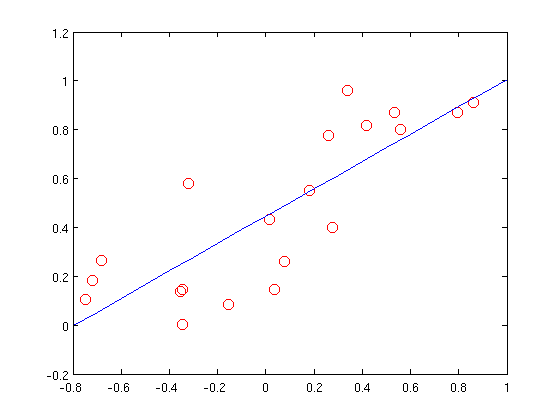
\includegraphics[width=6cm]{img/fit.png}
\end{center}

\subsection{Regressão}

Podemos calcular automaticamente um modelo de regressão (usando quadrados mínimos) através da janela de um gráfico.

Exemplo:
\codigotikz{>> & load census\\
  >> & plot(cdate, pop, 'ro')}

Na janela do gráfico, podemos selecionar
\begin{center}
  Tools $\rightarrow$ Basic Fitting
\end{center}

Podemos calcular a norma dos resíduos para um \emph{fit} realizado através do comando
\codigotikz{>> & sqrt(sum(resids.\^{}2))}

Podemos também extrapolar dados usando a interface gráfica do MATLAB, novamente em 
\begin{center}
  Tools $\rightarrow$ Basic Fitting
\end{center}
Finalmente, podemos usar o comando 
\begin{center}
  File $\rightarrow$ Generate Code
\end{center}
para criarmos uma função que reproduz o gráfico obtido.

Alternativamente, o comando
\codigotikz{>> & p = polyfit(x,y,n)}
encontra os coeficientes do polinômio $p(x)$ de grau $n$ que aproxima os dados $y(i)=p(x(i))$, em um sentido de mínimos quadrados. O vetor \code{p} resultante contém os coeficientes do polinômio em ordem descendente de potências.

O comando
\codigotikz{>> &[p,S] = polyfit(x,y,n)}
retorna os coeficientes do polinômio em \code{p} e uma estrutura \code{S} que pode ser usada com o comando \code{polyval}. 

A estrutura \code{S} contém os campos \code{R}, \code{df} e \code{normr}.

Se os dados \code{y} são aleatórios, uma estimativa da covariância de \code{p} é
\codigotikz{>> & (inv(R)*inv(R)')*normr\^{}2/df}

O comando
\codigotikz{>> & y = polyval(p,x)}
retorna o valor de um polinômio de grau \code{n} (armazenado no vetor \code{p}) em \code{x}.
O comando 
\codigotikz{>> & [y,delta] = polyval(p,x,S)}
usa a estrutura \code{S} gerada pelo comando \code{polyfit} para gerar \code{delta}, que é uma estimativa do desvio padrão do erro obtido ao se tentar calcular \code{p(x)}. 

Exemplo: Se quisermos fazer uma regressão linear em um conjunto de pontos $(x,y)$, usamos o comando
\codigotikz{>> & p = polyfit(x,y,1)}
O resultado é um vetor \code{p} que contém os coeficientes da reta
$$y = p_1x+p_2$$

Exemplo:
\codigotikz{>> & x = 1:1:20;\\
  >> & y = x + 10*rand(1,20);\\
  >> & p = polyfit(x,y,1);\\
  >> & plot(x,y,'ro')\\
  >> & hold on\\
  >> & t = 0:0.1:20;\\
  >> & plot(t,polyval(p,t))}

Exemplo (com resíduos):
\codigotikz{>> & x = 1:1:20;\\
  >> & y = x + 10*rand(1,20);\\
  >> & p = polyfit(x,y,1);\\
  >> & fitted = polyval(p,x);\\
  >> & res = y-fitted;\\
  >> & subplot(2,1,1), plot(x,y,'ro','markersize',8)\\
  >> & hold on\\
  >> & t = 0:0.1:20;\\
  >> & subplot(2,1,1), plot(t,polyval(p,t))\\
  >> & subplot(2,1,2), bar(x,res)}  

O comando
\codigotikz{>> & scatter(X,Y)}
faz um gráfico dos pontos com coordenadas \code{X} e \code{Y}, usando círculos como marcadores.
   
Se usarmos
\codigotikz{>> & scatter(X,Y,S,C)}
podemos especificar a área de cada marcador em \code{S}. 

Outras opções:
\begin{itemize}
\item \code{scatter(...,marcador)} usa o marcador escolhido (p. ex. \code{'+'} ou \code{'*'})
\item \code{scatter(...,'filled')} preenche os marcadores.
\end{itemize}

O comando
\codigotikz{>> & scatterhist(x,y)}
cria um \emph{scatter plot} dos dados nos vetores \code{x} e \code{y} e também um histograma em cada eixo do gráfico. 

Exemplo: 
\codigotikz{>> & x = randn(1000,1);\\
  >> & y = exp(.5*randn(1000,1));\\
  >> & scatterhist(x,y)}

O comando
\codigotikz{>> & lsline}
acrescenta uma reta calculada através de regressão linear (mínimos quadrados) \emph{para cada plot/scatter plot na figura atual}. 

\paragraph*{Atenção:} dados conectados com alguns tipos de reta (\code{'-'}, \code{'--'} ou \code{'.-'}) são \emph{ignorados} por \code{lsline}.

Exemplo:
\codigotikz{>> & x = 1:10;\\
  >> & y1 = x + randn(1,10);\\
  >> & scatter(x,y1,25,'b','*')\\
  >> & hold on\\
  >> & y2 = 2*x + randn(1,10);\\
  >> & plot(x,y2,'mo')\\
  >> & y3 = 3*x + randn(1,10);\\
  >> & plot(x,y3,'rx:')\\
  >> & y4 = 4*x + randn(1,10);\\
  >> & plot(x,y4,'g+--')\\
  >> & lsline}

Se o vetor \code{p} contém os coeficientes de um polinômio em ordem descendente de potências, o comando
\codigotikz{>> & refcurve(p)}
adiciona uma curva de referência polinomial com coeficientes \code{p} ao gráfico atual.

Se \code{p} é um vetor com $n+1$ elementos, a curva é dada por
\begin{equation*}
  y = p(1)x^n + p(2)x^{n-1} + \ldots + p(n)x + p(n+1)
\end{equation*}

O comando
\codigotikz{>> & gline}
permite ao usuário adicionar manualmente um segmento de reta à última figura desenhada.

A reta pode ser editada manualmente na ferramenta de edição de gráficos do MATLAB.

\subsection{Comandos em Toolboxes}

Se sua instalação do MATLAB possuir a Statistics Toolbox, o comando
\codigotikz{>> & polytool(x,y)}
ajusta uma reta aos vetores \code{x} e \code{y} e mostra um gráfico interativo do resultado.
\codigotikz{>> & polytool(x,y,n)}
ajusta um polinômio de grau \code{n} aos dados.

Se sua instalação possuir a Curve Fitting Toolbox, você pode fazer o ajuste de curvas de maneira interativa, usando o comando 
\codigotikz{>> & cftool}
 
\chapter{Resolução de equações lineares e não-lineares com MATLAB}

Neste capítulo, vamos ver um apanhado dos comandos mais utilizados para a resolução de sistemas lineares, resolução de equações não-lineares e de sistemas não-lineares de equações.

\section{Comandos básicos de álgebra linear}

Primeiramente, vamos ver alguns comandos básicos para matrizes:
\begin{itemize}
\item Para calcularmos o determinante de uma matriz quadrada \code{A}, usamos o comando
  \codigotikz{>> & det(A)}
\item Para calcularmos os autovalores e autovetores de uma matriz quadrada \code(A), usamos o comando \code{eig(A)}.
\item Se digitarmos simplesmente
  \codigotikz{>> & eig(A)}
  o resultado é um vetor contendo os autovalores de $A$. Se usarmos a forma
  \codigotikz{>> & [V,D] = eig(A)}
  o resultado é uma matriz \code{V} cujas colunas são autovetores de $A$, e uma matriz diagonal \code{D} cujos elementos não nulos são os autovalores de $A$.
\item Para calcularmos a inversa de uma matriz \emph{quadrada e inversível} \code{A}, usamos o comando
  \codigotikz{>> & inv(A)}
\end{itemize}	

\section{Resolução de Sistemas Lineares no MATLAB}

Aqui, vamos supor que queremos resolver um sistema linear, ou seja, um problema do tipo 
	
\begin{center}
  \begin{tikzpicture}
    \node[draw, rectangle, rounded corners, thick] {\begin{minipage}{0.5\textwidth} \begin{center} Encontrar $x\in {\mathbb{R}}^n$ tal que \begin{equation*} Ax=b\end{equation*} com $A\in {\mathbb{R}}^{m\times n}$ e $b\in {\mathbb{R}}^m$.\end{center}\end{minipage}};
  \end{tikzpicture}
\end{center}

Existem algumas maneiras de resolver este tipo de problema no MATLAB. 
	
\subsection{Usando a inversa: \code{inv}}
	
Primeiramente, se $m=n$ (ou seja, a matriz do problema é quadrada) e $A$ for inversível, podemos simplesmente invertê-la para encontrar
\begin{equation*}
   x = A^{-1}b.
\end{equation*}
No MATLAB, teremos então
\codigotikz{>> & x = inv(A)*b}
No entando, sabemos que esse método é o menos eficiente de todos, tanto em desempenho quanto em termos de instabilidade numérica. Assim, vamos procurar outros métodos para resolvermos esse problema.
	
\subsection{O operador \code{\textbackslash}}
	
Se, não for desejável encontrar a inversa da matriz $A$, ou se ela não for quadrada, e não quisermos nos preocupar com o método utilizado na resolução do sistema (em outras palavras, estamos interessados em uma solução, mesmo que aproximada, e não no método utilizado para a resolução), podemos usar o operador \code{\textbackslash} no MATLAB. Para nosso sistema $Ax=b$, teríamos então
\codigotikz{>> & x = A\textbackslash b}

Este operador atua da seguinte maneira:
\begin{itemize}
  \item Se $A$ for quadrada e inversível, então $x$ é a solução do sistema encontrada por \code{x = inv(A)*b}. 
  \item Se $A$ for quadrada, mas não for inversível, uma mensagem de erro é mostrada. O MATLAB tentará resolver o sistema, mas o resultado obtido nem sempre é confiável. Você pode verificar isso avaliando o resíduo, que pode ser bastante grande em casos de mal condicionamento extremo.
  \item Se $A$ for $m\times n$ com $m\ne n$, então $x$ é a solução no sentido de mínimos quadrados do sistema, ou seja, $x$ minimiza a norma do resíduo $r = \norm{Ax-b}$. 
\end{itemize}

\subsection{Decomposição LU: \code{lu}}

Sabe-se da álgebra linear que se for possível encontrar a decomposição LU de uma matriz $A$, é possível resolver o sistema $Ax=b$ através de dois sistemas triangulares, um superior e um inferior, da seguinte forma:
\begin{equation*}
   Ax=b \Leftrightarrow (LU)x=b \Leftrightarrow \left\{ \begin{array}{r c l}
         Ly &=&b\\Ux &=& y\end{array} \right.	   
\end{equation*}
	
Para encontrarmos a decomposição LU de uma matriz $A$ no MATLAB, usamos o comando
\codigotikz{>> & [L,U] = lu(A)}
Podemos em seguida resolver o sistema $Ax=b$ fazendo
\codigotikz{>> & y = L\textbackslash b\\>> & x = U\textbackslash y}
	
\subsection{\code{linsolve}}
	
Se não quisermos nos preocupar com o algoritmo usado na resolução do sistema, temos uma outra opção no comando \code{linsolve}.
\codigotikz{>> & x = linsolve(A,b)}
resolve o sistema linear $Ax=b$ usando a fatoração LU com pivotamento parcial de $A$, caso a matriz seja quadrada, e a fatoração QR de
$A$ com pivotamento nas colunas, caso contrário.

\subsection{Métodos Iterativos para Sistemas Lineares}

O MATLAB também conta com alguns algoritmos para resolver sistemas lineares de forma iterativa, isto é, a partir de um ponto inicial $x_0$, obtém-se uma aproximação para a solução exata do sistema através da realização de algum procedimento várias vezes, até que alguma condição seja satisfeita. 

Se a matriz $A$ for grande e esparsa, métodos diretos (usando fatoração) são, em geral, pouco eficientes. Nestes casos, podemos usar um dos seguintes métodos, disponíveis no MATLAB:

\begin{itemize}
   \item \code{pcg} Gradiente conjugado precondicionado
   \item \code{bicg} Gradiente bi-conjugado (gradiente conjugado para matrizes não necessariamente simétricas)
   \item \code{gmres} Generalized minimum residual method (com restarts)
   \item \code{lsqr} LSQR (quadrados mínimos)
\end{itemize}

Para mais informações sobre estes métodos, pode-se consultar no \emph{help} do MATLAB a página intitulada \emph{Systems of Linear Equations}, no item \emph{Iterative Methods for Solving Systems of Linear Equations}.

\section{Resolução de equações não-lineares}

\subsection{Equação não linear a uma variável: \code{fzero}}

Aqui, o problema que nos interessa é encontrar uma raiz da equação
\begin{equation*}
   f(x)=0
\end{equation*}
onde $f$ é uma função de uma variável real. Para encontrarmos a solução deste problema para uma função $f$ qualquer, a partir de um ponto $x0$, podemos usar o comando \code{fzero(função,x0)}. No entanto, um cuidado especial com a função a ser minimizada é necessário.

No MATLAB, para passarmos uma função como argumento de outra função (no caso, queremos passar $f(x)$ como argumento da função \code{fzero}) precisamos obter a \emph{referência} da função (assim como tínhamos obtido a referência a um objeto gráfico anteriormente). 

Primeiramente, a função para a qual gostaríamos de encontrar uma raiz deve estar em um arquivo próprio, definida como uma função do MATLAB, no formato
\codigotikz{[y] &= minhafuncao(x)\\
   & comandos}

Em seguida, chamamos a função \code{fzero} no console para minimizar a função \code{minhafuncao} a partir do ponto \code{x0}, escrevendo
\codigotikz{>> & fzero(@minhafuncao,x0)}
	
Exemplo:
   Para encontrar uma das raizes de $f(x) = x^2-4$, previamente definida em um arquivo de nome \code{quadratica.m}, a partir do ponto $x=6$, usamos o comando 
   \codigotikz{>> fzero(@quadratica,6)}
 
O algoritmo da função \code{fzero} usa uma combinação dos métodos da bissecção, secante e interpolação quadrática inversa.	
	
\subsection{Raizes de um polinômio: \code{roots}}
        
Para encontrar as raizes de um polinômio de grau $n$ da forma
\begin{equation*}
   p(x) = a_0+a_1x+a_2x^2+\ldots+a_nx^n
\end{equation*}
primeiramente representamos este polinômio como um vetor \emph{linha} \code{p} no MATLAB, cujas componentes são os coeficientes dos termos em ordem descendente de grau, ou seja,
\codigotikz{>> & p = [a$_n$ a$_{n-1}$ $\cdots$ a$_2$ a$_1$ a$_0$]}
Em seguida, usamos o comando
\codigotikz{>> & r = roots(p)}
resultando em um vetor coluna \code{r} com as raizes deste polinômio.

Exemplo:
   $p(x) = t^3+2t^2-5t-6$ (Figura \ref{fig:polinomio}).
   \codigotikz{>> & p = [1 2 -5 -6]\\
      >> & roots(p)}
   \begin{figure}
      \begin{center}
         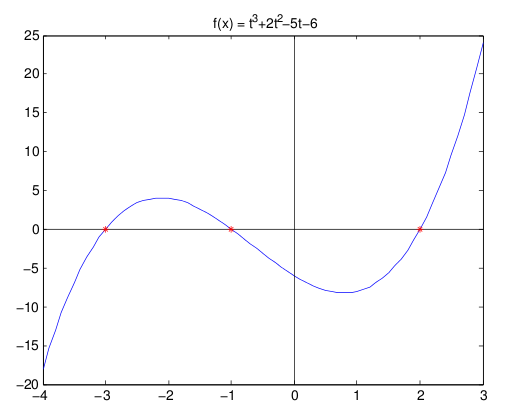
\includegraphics[width=6cm]{img/polinomio.png}
         \label{fig:polinomio}
         \caption{$p(x) = t^3+2t^2-5t-6$ e suas raizes.}
      \end{center}
   \end{figure}
 
\subsection{Sistema de equações não lineares: \code{fsolve}}

Para encontrarmos a solução de um sistema de equações não lineares da forma
\begin{equation*}
   F(x) = 0
\end{equation*}
onde $F:{\mathbb{R}}^n \rightarrow {\mathbb{R}}^m$, usamos a função \code{fsolve}. Neste caso, similarmente à função \code{fzero}, devemos escrever a função $F(x)$ em um arquivo \code{.m} separadamente, e usar a sintaxe
\codigotikz{>> & fsolve(@minhafuncao,x0)}

Exemplo: Resolver o sistema de equações 
   \begin{equation*}
      \left\{ \begin{array}{r c l}
            y_1 &=& 3x_1^2+4x_2^2-16\\
            y_2 &=& 2x_1^2-3x_2^2-5
         \end{array} \right.
   \end{equation*}
   \codigotikz{>> & fsolve(@funcs,[1;1])}
 
\paragraph*{Observação} Este comando faz parte da \emph{Optimization Toolbox}, que pode não estar disponível na sua instalação do MATLAB.
	
\section{Otimização: Minimização de funções}
	
Agora, queremos resolver o problema
\begin{equation*}
   \mbox{ minimizar } f(x).
\end{equation*}
   
\subsection{Minimização de uma função de uma variável: \code{fminbnd}}

Para encontrarmos o mínimo de uma função de uma variável dentro de um intervalo $[a,b]$, usamos o comando
\codigotikz{>> & x = fminbnd(@funcao,a,b)}
Se quisermos também saber o valor da função no ponto de mínimo, usamos a sintaxe
\codigotikz{>> & [x,fval] = fminbnd(@funcao,a,b)}

\subsection{Minimização de uma função de várias variáveis: \code{fminsearch}}

Para encontrarmos o mínimo de uma função real de várias variáveis, a partir de um ponto inicial \code{x0}, usamos o comando
\codigotikz{>> & x = fminsearch(@funcao,x0)}
Se quisermos também saber o valor da função no ponto de mínimo, usamos a sintaxe
\codigotikz{>> & [x,fval] = fminsearch(@funcao,x0)}

\chapter{Outros comandos úteis}

\section{Interpolação polinomial: \code{interpn}}

Para interpolarmos um conjunto de pontos em 1D, 2D, 3D ou em $n$ dimensões, usamos os comandos
\begin{itemize}
   \item \code{interp1}
   \item \code{interp2}
   \item \code{interp3}
   \item \code{interpn}
\end{itemize}
respectivamente.   

\subsection{Interpolação 1D: \code{interp1}}

O comando
\codigotikz{>> & yi = interp1(x,Y,xi,method)}
interpola os dados (\code{x},\code{Y}) nos novos pontos \code{xi}, usando o método \code{method}, que pode ser:
\begin{itemize}
   \item \code{'nearest'} Vizinho mais próximo
   \item \code{'linear'} Interpolação linear (default)
   \item \code{'spline'} Splines cúbicos
   \item \code{'cubic'} Interpolação por polinômios de Hermite
\end{itemize}

Exemplo:
   \codigotikz{>> & x = 0:10;\\
      >> & y = sin(x); \\
      >> & xi = 0:.25:10; \\
      >> & yi = interp1(x,y,xi); \\
      >> & plot(x,y,'o',xi,yi);\\
      >> & hold on;\\
      >> & zi = interp1(x,y,xi,'nearest');\\
      >> & plot(xi,zi,':k');\\
      >> & wi = interp1(x,y,xi,'spline');\\
      >> & plot(xi,wi,'m');\\
      >> & ui = interp1(x,y,xi,'cubic');\\
      >> & plot(xi,ui,'--g')
   }
   
\subsection{Interpolação 2D: \code{interp2}}

O comando
\codigotikz{>> & ZI = interp2(X,Y,Z,XI,YI,method)}
interpola os dados (\code{X},\code{Y},\code{Z}) nos novos pontos (\code{XI},\code{YI}) usando o método \code{method}, que pode ser
\begin{itemize}
   \item \code{'nearest'} Vizinho mais próximo
   \item \code{'linear'} Interpolação linear (default)
   \item \code{'spline'} Splines cúbicos
   \item \code{'cubic'} Interpolação cúbica, se os dados forem uniformemente
   espaçados; senão, é o mesmo que \code{spline}.
\end{itemize}

\section{Aproximação polinomial: \code{polyfit}}

O comando
\codigotikz{>> & p = polyfit(x,y,n)}
encontra os coeficientes do polinômio $p(x)$ de grau $n$ que aproxima os dados $y(i)=p(x(i))$, em um sentido de mínimos quadrados. O vetor \code{p} resultante contém os coeficientes do polinômio em ordem descendente de potências.

Exemplo:
   Tentar interpolar com um polinômio os mesmos pontos do exercício anterior, ou seja, 
   \codigotikz{>> & x = 0:10;\\
      >> & y = sin(x);}
 
\section{Integração Numérica}

\subsection{Integração numérica geral: \code{integral}}

Para calcularmos uma aproximação numérica de $\int_a^b f(x) dx$, usamos o comando
\codigotikz{>> & q = integral(fun,a,b)}
em que \code{fun} é uma referência a uma função.

Exemplo:
   Calcular a integral imprópria $f(x) = e^{-x^2}(\ln{(x)})^2$ entre $0$ e $\infty$.
   \codigotikz{>> & fun = @(x) exp(-x.\^{}2).*log(x).\^{}2;\\
      >> & q = integral(fun,0,Inf)
   }
 
\subsection{Integração numérica finita: \code{quad}}

Para calcularmos uma aproximação numérica de $\int_a^b f(x) dx$ com $a$ e $b$ finitos pela quadratura de Simpson (adaptativa), usamos o comando
\codigotikz{>> & q = quad(fun,a,b)}
em que \code{fun} é uma referência a uma função.

\subsection{Integração numérica discreta: \code{trapz}}

Se tudo o que conhecemos sobre a função é seus valores em um conjunto de pontos, podemos aproximar o valor da sua integral $\int_a^b f(x) dx$ usando o comando \code{trapz}:
\codigotikz{>> & x = 0:pi/100:pi;\\
   >> & y = sin(x);\\
   >> & z = trapz(x,y)}

\section{Diferenciação Numérica: \code{gradient}}

O \emph{gradiente} de uma função $f:{\mathbb{R}}^n \to {\mathbb{R}}$ é dado por
\begin{equation*}
  \nabla f(x) = \left( \frac{\partial f}{\partial x_1}(x), \frac{\partial f}{\partial x_1}(x), \ldots, \frac{\partial F}{\partial x_n}(x)\right).
\end{equation*}

Para calcularmos o gradiente de uma função de uma variável, procedemos da seguinte maneira.

\codigotikz{>> & x = a:h:b;\\
  >> & f = funcao(x);\\
  >> & g = gradient(f,h)}

O comando \code{gradient} calcula numericamente a derivada de $f$ em função da variável $x$ nos pontos escolhidos. 

Para calcularmos o gradiente de uma função de duas variáveis, o procedimento é equivalente. A diferença é que agora precisamos gerar uma malha de pontos usando o comando \code{meshgrid}.

\codigotikz{>> & x = a:hx:b;\\
  >> & y = c:hy:d;\\
  >> & [x,y] = meshgrid(x,y);\\
  >> & f = funcao(x,y)\\
  >> & [gx,gy] = gradient(f,hx,hy)}

\section{Resolução de Equações Diferenciais Ordinárias}

\subsection{Problemas de Valor Inicial}

Uma equação diferencial ordinária (EDO) é uma equação que envolve uma ou mais derivadas de uma variável dependente $y$ com respeito a uma única variável independente $t$ ($y = y(t)$). Com frequência, $y(t)$ é um vetor com componentes $y = (y_1(t), y_2(t), \ldots, y_n(t))$.

O MATLAB resolve equações diferenciais ordinárias de primeira ordem dos seguintes tipos:
\begin{itemize}
\item EDOs explícitas, do tipo $y' = f(t,y)$
\item EDOs linearmente implícitas, do tipo $M(t,y)y' = f(t,y)$, em que $M(t,y)$ é uma matriz
\item EDOs implícitas, do tipo $f(t,y,y') = 0$ %(ode15i only)
\end{itemize}

Para resolvermos equações diferenciais de ordem superior, precisamos escrevê-las como um sistema de equações de primeira ordem (como fazemos no curso de cálculo).

Geralmente, temos uma família de soluções $y(t)$ que satisfaz a EDO. Para obtermos uma solução única, exigimos que a solução satisfaça alguma condição inicial específica, de forma que $y(t_0) = y_0$ em algum valor inicial $t_0$.
\begin{align*}
  y' = f(t,y)\\
  y(t_0) = y_0
\end{align*}

No MATLAB, temos solvers para três tipos de problemas de valor inicial. Em todos os casos, a sintaxe para resolver uma equação diferencial é
\codigotikz{>> & [t,y] = solver(odefun,tspan,y0,options)}
onde \code{solver} é substituido por uma das opções que veremos em seguida. Os argumentos de entrada são sempre os seguintes:
\begin{itemize}
  \item \code{odefun}: O \emph{handle} para uma função que avalia o sistema de EDOs em um ponto. Esta função deve estar na forma \code{dydt = odefun(t,y)}, onde \code{t} é um escalar e \code{dydt} e \code{y} são vetores coluna.
  \item \code{tspan}: vetor especificando o intervalo de integração. O solver impõe a condição inicial em \code{tspan(1)}, e integra de \code{tspan(1)} até \code{tspan(end)}.
  \item \code{y0}: vetor das condições iniciais para o problema.
  \item \code{options}: Struct de parâmetros opcionais que modificam as propriedades padrão de integração.
\end{itemize}

Os argumentos de saída são
\begin{itemize}
\item \code{t}: vetor coluna das variáveis independentes (pontos no intervalo desejado)
\item \code{y}: vetor ou matriz contendo, em cada linha, a solução calculada no ponto contido na linha correspondente de \code{t}.
\end{itemize}

\subsection{Solvers}

Os métodos disponíveis estão divididos de acordo com o tipo de problema que resolvem:
\begin{itemize}
\item Problemas Não-Stiff:
  \begin{itemize}
  \item \code{ode45} (Runge-Kutta, passo simples)
  \item \code{ode23} (Runge-Kutta, passo simples)
  \item \code{ode113} (Adams-Bashforth-Moulton, passo múltiplo)
  \end{itemize}
\item Problemas Stiff:
  \begin{itemize}
  \item \code{ode15s} (numerical differentiation formulas (NDFs), passo múltiplo)
  \item \code{ode23s} (Rosenbrock, passo único)
  \item \code{ode23t} (Trapezoide)
  \item \code{ode23tb} (Runge-Kutta)
  \end{itemize}
\end{itemize}

Para equações implícitas da forma
\begin{equation*}
  f(t,y,y') = 0, 
\end{equation*}
pode-se usar o solver \code{ode15i} (consultar a documentação para mais detalhes).

\end{document}

